\section{Hệ sinh thái dữ liệu và Data Warehouse}
\subsection{Tổng quan về dữ liệu}
Trong kiến trúc của hệ thống Thông tin Giao thông Thông minh (Traffic IoC), Data Pipeline không chỉ đơn thuần đóng vai trò truyền tải dữ liệu, mà hoạt động như một lớp hạ tầng cốt lõi đảm bảo tính nhất quán, độ tin cậy và khả năng sẵn sàng của Data Warehouse. Dữ liệu giao thông đặc thù mang tính chất chuỗi thời gian (time-series) kết hợp với dữ liệu không gian (spatial data), đòi hỏi một luồng xử lý cực kỳ nghiêm ngặt trước khi được lưu trữ vào hệ quản trị cơ sở dữ liệu PostgreSQL có tích hợp PostGIS.


Toàn bộ luồng xử lý được chuẩn hóa theo mô hình ETL ba pha độc lập: Extract (Trích xuất) → Transform (Biến đổi) → Load (Nạp). Điểm đột phá của kiến trúc này nằm ở nguyên lý Separation of Concerns (Tách biệt mối quan tâm). Mỗi pha trong chu trình được giao phó một trách nhiệm duy nhất và không can thiệp vào logic của các pha khác. Extractor chỉ giao tiếp với API bên ngoài; Transformer đảm nhiệm việc áp dụng các quy tắc nghiệp vụ; Loader chịu trách nhiệm đóng gói và thực thi các giao dịch (transactions) vào cơ sở dữ liệu. Cách tiếp cận này giúp hệ thống đạt được tính mô-đun hóa (modularity) cao, dễ dàng bảo trì, mở rộng quy mô (scale) và cho phép tích hợp các nguồn dữ liệu mới mà không làm phá vỡ cấu trúc hiện tại.

\subsubsection{Các nguồn dữ liệu chính}
Phần này tập trung tìm hiểu và phân tích các nguồn data input, bao gồm 3 nguồn chính sau: TomTom, Google Maps và OpenStreetMap để xác thực độ khả thi của thiết kế tại mục 5.1.2, qua đó điều chỉnh để tính khả thi đạt 100\%.

\subsubsubsection{TomTom}

\textbf{Các loại dữ liệu và phạm vi cung cấp:} TomTom cung cấp một hệ sinh thái dữ liệu giao thông toàn diện, bao gồm cả dữ liệu thời gian thực (Real-time) với tần suất cập nhật mỗi phút và dữ liệu lịch sử phục vụ thống kê. Các nhóm dữ liệu chính bao gồm:
\begin{itemize}
    \item \textbf{Dữ liệu dòng giao thông (Traffic Flow):} Cung cấp các chỉ số về tốc độ quan sát thực tế (observed speed), thời gian di chuyển (travel time) và so sánh với tốc độ dòng chảy tự do (free-flow) cho từng phân đoạn đường (road segments).
    \item \textbf{Sự cố giao thông (Traffic Incidents):} Thông tin chi tiết về các sự kiện gây cản trở giao thông như tai nạn, công trường thi công, hoặc đường đóng. Dữ liệu bao gồm vị trí bắt đầu/kết thúc, độ dài đoạn ảnh hưởng, loại sự cố và mức độ nghiêm trọng.
    \item \textbf{Dữ liệu hiển thị và điều khiển:} Hỗ trợ các lớp bản đồ Vector Tiles cho luồng giao thông và sự cố, cùng với thông tin cập nhật giới hạn tốc độ động (Live speed restrictions) giúp tăng cường độ chính xác cho các ứng dụng dẫn đường.
\end{itemize}

\textbf{Cấu trúc và định dạng dữ liệu kỹ thuật:} Về mặt kỹ thuật, TomTom sử dụng các chuẩn dữ liệu phổ biến để đảm bảo tính tương thích cao.
\begin{itemize}
    \item Các phản hồi từ REST API (như thông tin sự cố, metadata, lỗi) được trả về dưới định dạng \textbf{JSON} tiêu chuẩn.
    \item Đối với các dữ liệu yêu cầu hiệu năng hiển thị cao như Flow/Incident Tiles, TomTom sử dụng định dạng vector nhị phân (\textbf{Binary Protobuf/PBF-like}), được tuần tự hóa bởi Google Protocol Buffers theo schema riêng.
    \item Các trường thông tin (key fields) quan trọng phục vụ cho việc mô hình hóa dữ liệu bao gồm: tọa độ không gian (\texttt{start/endLocation}), tên đường (\texttt{roadName}), tham số giao thông (\texttt{delay}, \texttt{speedObserved}, \texttt{speedFreeFlow}), độ tin cậy của dữ liệu (\texttt{confidence}) và nhãn thời gian (\texttt{timestamp}).
\end{itemize}

\textbf{Cơ chế truy cập và Chính sách sử dụng:} Để tích hợp vào hệ thống, nhà phát triển cần đăng ký API Key thông qua TomTom Developer Portal. Dữ liệu được truy xuất thông qua các RESTful API endpoints (như Traffic Incidents service) hoặc Vector Tile endpoints.
\begin{itemize}
    \item Về mặt giới hạn và chi phí, TomTom áp dụng mô hình giới hạn truy cập (Rate limits) dựa trên từng khóa API hoặc gói dịch vụ cụ thể.
    \item Mô hình chi phí dựa trên mức độ sử dụng (pay-as-you-go). Đáng chú ý, độ trễ dữ liệu (latency) được duy trì ở mức thấp, cập nhật từng phút, phù hợp cho các bài toán điều hướng thời gian thực.
\end{itemize}

\textbf{Đánh giá khả năng ứng dụng tại TP.HCM:}
\begin{itemize}
    \item \textbf{Ưu điểm:} Dữ liệu có độ tin cậy cao, cập nhật nhanh (real-time), hỗ trợ Vector Tiles giúp việc hiển thị và streaming dữ liệu lên bản đồ số mượt mà, hiệu quả. Đây là nguồn dữ liệu lý tưởng cho các ứng dụng yêu cầu độ chính xác cao như điều phối xe hoặc dẫn đường.
    \item \textbf{Nhược điểm và Thách thức:} Chi phí vận hành có thể tăng cao khi mở rộng quy mô (scale). Ngoài ra, độ phủ sóng dữ liệu (coverage) của TomTom tại TP.HCM chủ yếu tập trung tốt ở các đô thị lớn và đường trục chính; đối với hệ thống đường hẻm, đường nhánh nhỏ đặc thù của Việt Nam, lượng dữ liệu từ cảm biến/probe data có thể ít hơn.
\end{itemize}

\textbf{Kết luận:} Để tối ưu hóa hiệu quả và chi phí cho dự án, chiến lược đề xuất là chỉ sử dụng dữ liệu TomTom cho các tuyến đường trục chính, đường huyết mạch có vai trò quan trọng trong việc điều tiết giao thông toàn thành phố. Đối với các tuyến đường nhỏ hoặc hẻm không có tác động lớn đến luồng giao thông tổng thể, hệ thống sẽ cân nhắc sử dụng các nguồn dữ liệu thay thế.

\subsubsubsection{Google Maps}

\textbf{Các loại dữ liệu và phạm vi cung cấp:} Google Maps Platform cung cấp hệ sinh thái dữ liệu giao thông tập trung mạnh vào trải nghiệm dẫn đường và trực quan hóa.
\begin{itemize}
    \item \textbf{Dữ liệu giao thông thời gian thực (Real-time Traffic):} Cung cấp lớp hiển thị trực quan (\texttt{TrafficLayer}) trên bản đồ thông qua Maps JavaScript API.
    \item \textbf{Định tuyến và thời gian di chuyển (Traffic-aware Routing):} Thông qua \textbf{Directions API} và \textbf{Routes API} (\texttt{ComputeRoutes}), cung cấp ước lượng thời gian di chuyển chính xác dựa trên tình trạng giao thông thực tế.
    \item \textbf{Dữ liệu hạ tầng đường bộ:} \textbf{Roads API} hỗ trợ các tính năng như bám đường (snap-to-road), truy xuất giới hạn tốc độ (speed limits).
    \item \textbf{Lưu ý về sự cố giao thông:} Khác với TomTom, Google không cung cấp một luồng dữ liệu (feed) riêng biệt và có cấu trúc cho các sự cố (tai nạn, công trường) qua REST API.
\end{itemize}

\textbf{Cấu trúc và định dạng dữ liệu kỹ thuật:}
\begin{itemize}
    \item Các phản hồi từ REST API được trả về dưới định dạng \textbf{JSON}.
    \item Các trường thông tin quan trọng bao gồm: thời gian di chuyển trong điều kiện giao thông (\texttt{duration\_in\_traffic}), mô hình giao thông (\texttt{traffic\_model}), hình học tuyến đường (\texttt{geometry polyline}), phân đoạn hành trình (\texttt{legs/steps}) và giới hạn tốc độ (\texttt{speedLimits}).
    \item Dữ liệu có độ trễ thấp, phù hợp cao cho các tác vụ thời gian thực.
\end{itemize}

\textbf{Cơ chế truy cập và Chính sách sử dụng:} Việc truy cập dữ liệu được quản lý chặt chẽ thông qua Google Cloud Console, yêu cầu bắt buộc phải có API Key và tài khoản thanh toán (Billing account). Chi phí tính theo mô hình pay-as-you-go, khá cao cho các tính năng nâng cao như \texttt{ComputeRoutes} ở quy mô lớn.

\textbf{Đánh giá khả năng ứng dụng tại TP.HCM:}
\begin{itemize}
    \item \textbf{Ưu điểm:} Độ phủ dữ liệu (coverage) tại TP.HCM rất tốt nhờ lượng người dùng thiết bị di động khổng lồ. Khả năng tích hợp sâu với các SDK (Mobile, Web) hỗ trợ mạnh mẽ cho các bài toán định tuyến.
    \item \textbf{Nhược điểm và Thách thức:} Rào cản lớn nhất là \textbf{chi phí vận hành}. Mô hình tính phí trên mỗi yêu cầu (request-based) tạo ra gánh nặng tài chính lớn khi thu thập dữ liệu liên tục cho Data Warehouse. Ngoài ra, việc thiếu API cung cấp dữ liệu sự cố dưới dạng cấu trúc gây khó khăn cho việc thống kê tự động.
\end{itemize}

\textbf{Kết luận:} Do các hạn chế về chi phí và cấu trúc dữ liệu sự cố, Google Maps Platform được xếp độ \textbf{ưu tiên thấp nhất} trong việc làm nguồn dữ liệu đầu vào cho Kho dữ liệu. Nguồn này sẽ chỉ được cân nhắc sử dụng cho các chức năng hiển thị (Visual layer) ở phía người dùng cuối.

\subsubsubsection{OpenStreetMap}

\textbf{Các loại dữ liệu và phạm vi cung cấp:} OpenStreetMap (OSM) là cơ sở dữ liệu bản đồ nguồn mở toàn cầu. OSM cung cấp nền tảng dữ liệu địa lý tĩnh phong phú (mạng lưới đường bộ, ranh giới hành chính, POIs). Tuy nhiên, hệ thống \textbf{không cung cấp sẵn} dữ liệu lưu lượng giao thông thời gian thực hay thông tin sự cố tức thời.

\textbf{Cấu trúc và định dạng dữ liệu kỹ thuật:}
\begin{itemize}
    \item Dữ liệu OSM được tổ chức linh hoạt dựa trên mô hình thẻ (tags).
    \item Sử dụng \textbf{PBF (Protocolbuffer Binary Format)} cho lưu trữ offline và \textbf{OSM XML} hoặc \textbf{Overpass JSON} cho API.
    \item Các trường thông tin quan trọng: loại đường (\texttt{highway}), giới hạn tốc độ (\texttt{maxspeed}), chiều di chuyển (\texttt{oneway}), số làn xe (\texttt{lanes}), kết cấu mặt đường (\texttt{surface}).
\end{itemize}

\textbf{Cơ chế truy cập và Chính sách sử dụng:} OSM cung cấp cơ chế truy cập rất linh hoạt và mở (thông qua Geofabrik hoặc Overpass API). Dữ liệu hoàn toàn miễn phí dưới giấy phép \textbf{ODbL}. Chi phí thực tế chuyển dịch sang phần hạ tầng kỹ thuật (self-host) để tránh giới hạn truy cập.

\textbf{Đánh giá khả năng ứng dụng tại TP.HCM:}
\begin{itemize}
    \item \textbf{Ưu điểm:} Thế mạnh lớn nhất là độ chi tiết về hình học đường bộ, đặc biệt là hệ thống \textbf{đường hẻm, ngõ nhỏ} và lối đi bộ. Đây là nguồn dữ liệu nền tảng tuyệt vời để xây dựng đồ thị giao thông (topology graph).
    \item \textbf{Nhược điểm:} Thiếu dữ liệu traffic thời gian thực, không thể dùng độc lập để dự báo tắc nghẽn. Độ đồng nhất của dữ liệu thuộc tính tại ngoại ô có thể không cao.
\end{itemize}

\textbf{Kết luận:} OpenStreetMap là giải pháp tối ưu để giải quyết bài toán "phủ sóng" bản đồ tại các khu vực hẻm nhỏ của TP.HCM. Chiến lược đề xuất là sử dụng OSM làm \textbf{lớp bản đồ nền (Base Map)} và mạng lưới định tuyến cơ sở.

% Bảng so sánh
\begin{table}[H]
\centering
\caption{Bảng tóm tắt so sánh 3 nguồn dữ liệu}
\begin{tabular}{|p{3cm}|p{4cm}|p{4cm}|p{4cm}|}
\hline
\textbf{Tiêu chí} & \textbf{TomTom} & \textbf{Google Maps Platform} & \textbf{OpenStreetMap (OSM)} \\ \hline
Độ phủ (TP.HCM) & Rộng, commercial-grade; đường chính tốt. & Rất rộng; coverage cao ở đô thị lớn. & Geometries \& POI tốt ở khu vực cộng đồng active; mạnh về hẻm/chi tiết nhỏ. \\ \hline
Độ chính xác & Cao cho road attributes \& traffic metrics trên đường lớn. & Rất cao; enterprise-grade map + signals từ user base lớn. & Rất tốt về geometry; attribute completeness biến thiên. \\ \hline
Real-time & \textbf{Có} — real-time flow \& incident feeds (vector tiles). & \textbf{Có} — traffic-aware routing, TrafficLayer; không có incident feed công khai. & \textbf{Không} native. Cần tích hợp bên thứ ba. \\ \hline
Chi phí & Commercial — tốn phí tùy volume; pricing theo API. & Commercial — pay-as-you-go; tốn kém ở scale lớn. & \textbf{Miễn phí} (ODbL). Chi phí ở hạ tầng (hosting). \\ \hline
\end{tabular}
\end{table}

\subsection{Xây dựng và thiết kế hệ thống ETL trong đồ án}
Hệ thống ứng dụng triệt để các Design Pattern, đặc biệt là Template Method Pattern, thông qua việc xây dựng một bộ framework ETL nội bộ dựa trên các lớp trừu tượng (abstract classes). Ba lớp nền tảng bao gồm BaseExtractor, BaseTransformer và BaseLoader. Thay vì triển khai logic tuần tự (procedural) ở từng script đơn lẻ, mọi pipeline cụ thể bắt buộc phải kế thừa và tuân thủ giao diện (interface) mà lớp cha định nghĩa.


\subsubsection{BaseExtractor: Chuẩn hóa giao thức mạng và cơ chế chịu lỗi}
Lớp BaseExtractor hoạt động như một "resilience boundary" (ranh giới chịu lỗi) bảo vệ hệ thống khỏi các yếu tố bất định của mạng viễn thông và các dịch vụ API bên ngoài. Lớp này cung cấp một session HTTP dùng chung và chuẩn hóa các headers.


Về mặt học thuật, việc tích hợp thư viện tenacity vào lớp này thể hiện một thiết kế hệ thống bền bỉ (resilient system design). Thay vì để pipeline sụp đổ khi gặp độ trễ mạng hoặc lỗi HTTP tạm thời (như 429 Too Many Requests, 502 Bad Gateway), BaseExtractor tự động thực hiện cơ chế Retry with Backoff. Hệ thống được cấu hình để thử lại tối đa 3 lần với khoảng thời gian chờ cố định là 2 giây giữa các lần thử đối với các exception liên quan đến ConnectionError hoặc Timeout. Điều này giúp triệt tiêu các lỗi nhiễu (noise) ngắn hạn, tăng tỷ lệ thành công của các chu kỳ thu thập dữ liệu thời gian thực.


\subsubsection{BaseTransformer: Đảm bảo tính Toàn vẹn Dữ liệu bằng Pure Functions}
Trong kỹ nghệ phần mềm hiện đại, BaseTransformer áp dụng triết lý của Lập trình Hàm (Functional Programming) bằng cách định nghĩa các biến đổi dữ liệu dưới dạng Pure Functions (Hàm thuần túy). Lớp này hoàn toàn không có side-effect: không thực hiện I/O mạng, không truy vấn cơ sở dữ liệu và không ghi file. Nó chỉ nhận đầu vào là dữ liệu thô (raw data) và sinh ra đầu ra là một tập hợp các đối tượng (dictionaries) đã được chuẩn hóa.


Sự lựa chọn thiết kế này mang lại ba lợi ích lý luận sâu sắc:


Tính tất định (Determinism): Cùng một cấu trúc dữ liệu đầu vào tại bất kỳ thời điểm nào cũng sẽ luôn trả về một kết quả đầu ra giống hệt nhau.


Khả năng tái lập (Reproducibility): Khi xảy ra sự cố cần chạy lại pipeline (backfill), hệ thống có thể xử lý lại các tệp payload cũ mà không lo ngại về trạng thái (state) thay đổi làm sai lệch dữ liệu.


Khả năng kiểm thử cô lập (Isolated Testing): Các unit test cho Transformer không cần phải thiết lập các Mock Object phức tạp cho Database hay API, gia tăng đáng kể độ bao phủ mã (code coverage).


\subsubsection{BaseLoader: Trừu tượng hóa Chiến lược Nạp dữ liệu vào Data Warehouse}
BaseLoader đóng vai trò là một Database Gateway, ẩn giấu mọi sự phức tạp của quá trình đóng gói dữ liệu và quản lý giao dịch (transaction management). Kiến trúc này từ chối việc sử dụng các vòng lặp chèn dữ liệu (insert loops) thông thường để thay thế bằng việc chia lô (batching) và xử lý nguyên tử (atomic commits). Đặc biệt, BaseLoader có khả năng tự động nội suy cấu trúc bảng (table reflection) và hỗ trợ tự động sinh các phân vùng logic (table partitions) dựa trên trường date\_key, một kỹ thuật then chốt để tối ưu hóa hiệu suất truy vấn trong các hệ quản trị Big Data.

\subsection{Thiết kế Data Warehouse Schema}
\subsubsection{Phân tích nghiệp vụ nâng cao và xây dựng mô hình Galaxy Schema}

Nhóm nghiên cứu chuyển sang phân tích nghiệp vụ chuyên sâu và đề xuất mô hình \textbf{Galaxy Schema} – phù hợp khi nhiều quy trình nghiệp vụ chia sẻ chung một tập các bảng chiều chuẩn hóa.

\subsubsubsection{Phân tích ma trận nghiệp vụ}
Thông qua việc phân tích các nhóm nghiệp vụ từ BKTraffic, tài liệu liên quan, nhóm nhận thấy các luồng dữ liệu giao thông không tồn tại độc lập mà có mối quan hệ chặt chẽ với nhau. Các câu hỏi phân tích thực tế thường yêu cầu kết hợp dữ liệu từ nhiều nguồn khác nhau. Điều này làm nổi bật nhu cầu thiết kế mô hình dữ liệu tích hợp thay vì các Star Schema tách biệt.

\begin{table}[H]
\centering
\caption{Ma trận quy trình nghiệp vụ và các chiều dữ liệu}
\begin{tabular}{|l|c|c|c|c|c|c|}
\hline
\textbf{Quy trình nghiệp vụ} & \textbf{Time} & \textbf{Location} & \textbf{Vehicle} & \textbf{Weather} & \textbf{Incident} & \textbf{Source} \\ \hline
Theo dõi lưu lượng & X & X & X & X & & X \\ \hline
Giám sát sự cố & X & X & & X & X & X \\ \hline
Vận tải công cộng & X & X & X & & & \\ \hline
Dự báo thời tiết & X & X & & X & & \\ \hline
Điều phối tín hiệu & X & X & & & & X \\ \hline
\end{tabular}
\end{table}

Một số mối liên kết nghiệp vụ tiêu biểu:
\begin{itemize}
    \item Mối liên hệ giữa lưu lượng và an toàn giao thông\\
    Các nghiệp vụ như “Dự báo ùn tắc đa yếu tố” và “Đánh giá rủi ro theo khu vực” yêu cầu đồng thời thông tin về mật độ lưu thông (từ fact\_traffic\_flow) và thông tin sự cố, tai nạn (từ fact\_incident). Đây là dạng phân tích phức hợp, không thể thực hiện hiệu quả khi hai hệ thống tồn tại độc lập.
    \item Mối liên hệ giữa vận hành giao thông và yếu tố môi trường \\
    Nghiệp vụ “Dự báo giao thông theo điều kiện khí hậu” đòi hỏi tích hợp dữ liệu mưa, nhiệt độ, sương mù từ nguồn thời tiết (fact\_external\_condition) để giải thích sự biến động của tốc độ dòng xe hoặc mức độ ùn ứ.
    \item Mối liên hệ giữa sự kiện và nhu cầu giao thông\\
    Nghiệp vụ “Dự báo mật độ quanh khu vực sự kiện” yêu cầu liên kết dữ liệu về sự kiện đô thị (fact\_event) với hạ tầng giao thông, tuyến đường, phân đoạn và mật độ tại từng khu vực.

\end{itemize}

Kết quả phân tích cho thấy cần xây dựng tập Conformed Dimensions dùng chung để xóa bỏ tình trạng “ốc đảo dữ liệu”, đảm bảo các bảng fact có thể truy vấn và kết hợp dữ liệu đồng nhất.

\subsubsubsection{Thiết kế các Conformed Dimensions}

Để xử lý được các nghiệp vụ đa chiều và phức hợp, các bảng Dimension được tái cấu trúc với mức độ chuẩn hóa và hàm chứa ngữ nghĩa cao hơn đáng kể so với giai đoạn thiết kế ban đầu.\\

\textbf{1. Nhóm chiều Thời gian:}
Cung cấp trục thời gian đa cấp độ, liên kết toàn bộ các bảng Fact.
\begin{itemize}
    \item \texttt{dim\_date}, \texttt{dim\_date\_time}: Trục thời gian lịch và timestamp thực.
    \item \texttt{dim\_time\_of\_day}: Mô tả chi tiết 1.440 phút trong ngày, hỗ trợ bucket (5', 15').
    \item \texttt{dim\_shift}: Quản lý ca làm việc, giờ cao điểm.
    \item \texttt{dim\_holiday}, \texttt{bridge\_date\_holiday}: Quản lý ngày lễ, sự kiện đặc biệt.
\end{itemize}

\textbf{2. Nhóm chiều Không gian \& Hạ tầng:}
Hệ tọa độ chung mô tả cấu trúc phân cấp mạng lưới.
\begin{itemize}
    \item \texttt{dim\_segment}: Đơn vị cơ bản (phân đoạn đường giữa 2 node).
    \item \texttt{dim\_node}: Các nút giao, giao lộ.
    \item \texttt{dim\_route}, \texttt{bridge\_route\_segment}: Lộ trình và thứ tự segment.
    \item \texttt{dim\_way}, \texttt{dim\_road}: Cấp độ tuyến đường, trục chính.
\end{itemize}

\textbf{3. Nhóm chiều Đối tượng tham gia:}
\begin{itemize}
    \item \texttt{dim\_user}, \texttt{dim\_user\_detail}: Định danh và thuộc tính người dùng (SCD).
    \item \texttt{dim\_vehicle\_type}: Chuẩn hóa danh mục phương tiện (PCU, khí thải...).
\end{itemize}

\textbf{4. Nhóm chiều Ngữ cảnh \& Sự cố:}
\begin{itemize}
    \item \texttt{dim\_incident\_type}: Phân loại sự cố (tai nạn, ngập, công trình).
    \item \texttt{dim\_response\_unit}: Lực lượng phản ứng.
    \item \texttt{dim\_weather}: Thời tiết thực tế (mưa, gió, tầm nhìn).
\end{itemize}

\subsubsubsection{Thiết kế các bảng Fact theo nghiệp vụ}
Toàn bộ kiến trúc được tổ chức theo mô hình Galaxy Schema với 4 cụm nghiệp vụ:

\begin{itemize}
    \item \textbf{Cụm Vận hành Giao thông:}
    \begin{itemize}
        \item \texttt{fact\_traffic\_flow}: Lưu lượng tổng hợp, tốc độ trung bình, mức độ tắc nghẽn.
        \item \texttt{fact\_traffic\_flow\_by\_vehicle}: Lưu lượng chi tiết theo loại xe.
    \end{itemize}

    \item \textbf{Cụm Hành vi Người dùng:}
    \begin{itemize}
        \item \texttt{fact\_user\_travel\_time}: Hiệu suất di chuyển từng chuyến đi.
        \item \texttt{fact\_user\_mobility}: Thống kê hành vi tổng hợp.
    \end{itemize}

    \item \textbf{Cụm An toàn \& Sự cố:}
    \begin{itemize}
        \item \texttt{fact\_incident}: Ghi nhận sự cố, thời gian xử lý, mức độ nghiêm trọng.
    \end{itemize}

    \item \textbf{Cụm Hiệu quả Hệ thống:}
    \begin{itemize}
        \item \texttt{fact\_route\_recommendation}: Đánh giá hiệu quả gợi ý tuyến đường.
    \end{itemize}
\end{itemize}

\subsubsection{Tổng quan toàn bộ Galaxy Schema}
Mô hình Galaxy được xây dựng bằng cách sử dụng chung một tập hợp Dimensions chuẩn hóa. Tất cả các bảng Fact đều liên kết tới các Dimensions trong các chủ đề thời gian, không gian – hạ tầng, đối tượng tham gia và ngữ cảnh – sự cố, hình thành một cấu trúc phân tích đa chiều thống nhất.

\begin{figure}[H]
    \centering
    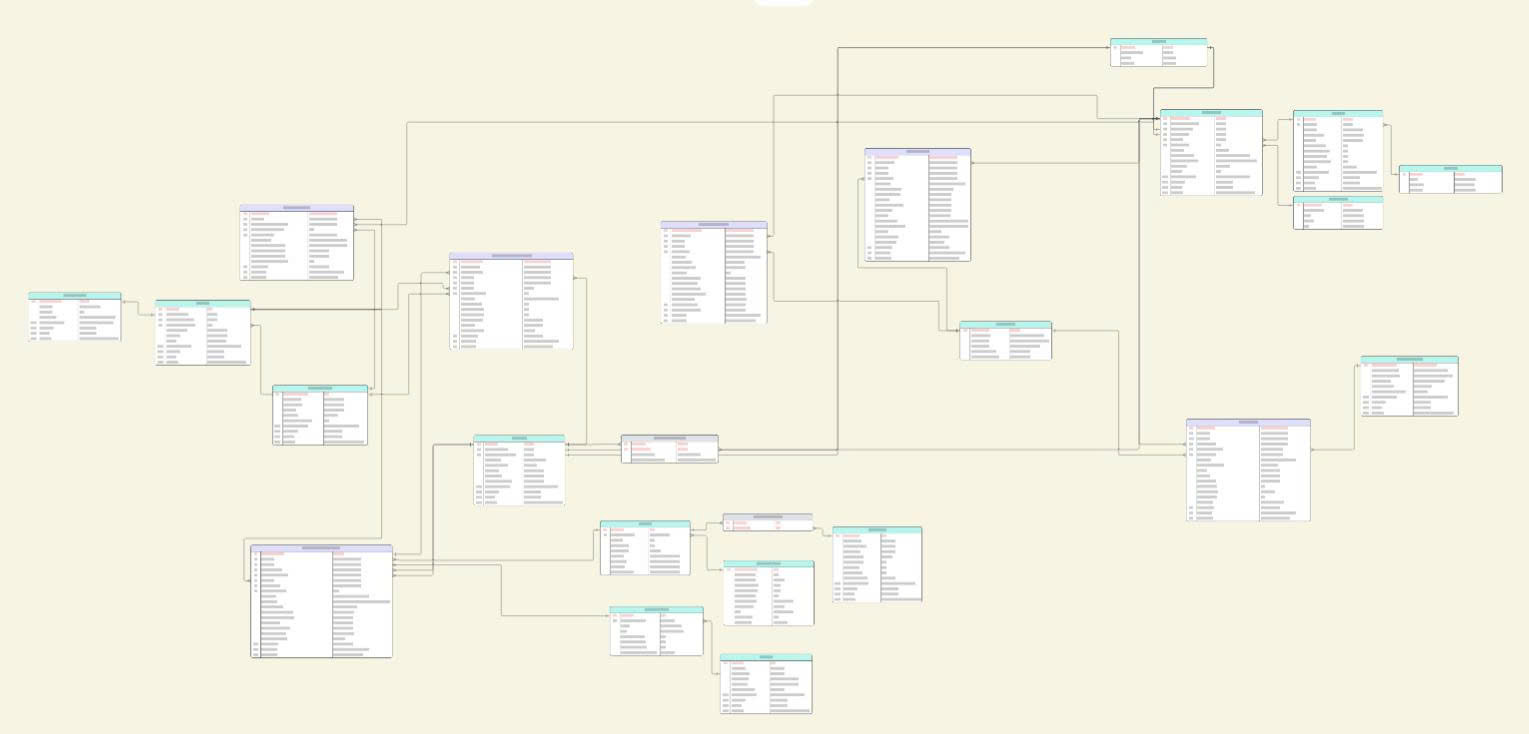
\includegraphics[width=1.0\textwidth]{Images/Picture5}
    \vspace{6mm}
    \caption{Mô hình Galaxy Schema hoàn chỉnh}
\end{figure}

\textbf{Các thành phần chính của hệ thống:}
\begin{itemize}
    \item \textbf{Hệ trục thời gian:} Bao trùm tất cả các Fact, hỗ trợ phân tích từ vi mô (phút) đến vĩ mô (năm).
    \item \textbf{Hệ tọa độ không gian – hạ tầng:} Cung cấp chuẩn tham chiếu không gian nhất quán (Segment $\rightarrow$ Node $\rightarrow$ Way $\rightarrow$ Road).
    \item \textbf{Hệ tham chiếu người dùng – phương tiện:} Phục vụ phân tích hành vi và tối ưu lộ trình.
    \item \textbf{Hệ ngữ cảnh – sự cố:} Then chốt trong phân tích an toàn và tác động môi trường.
\end{itemize}

Cách tổ chức này đảm bảo tính nhất quán dữ liệu, tăng khả năng phân tích chéo và sẵn sàng mở rộng cho các nguồn dữ liệu IoT trong tương lai.

\subsubsection{Bảng Fact}
Các ảnh bảng Fact với đầy đủ kết nối đến bảng Dim.

\begin{figure}[H]
    \centering
    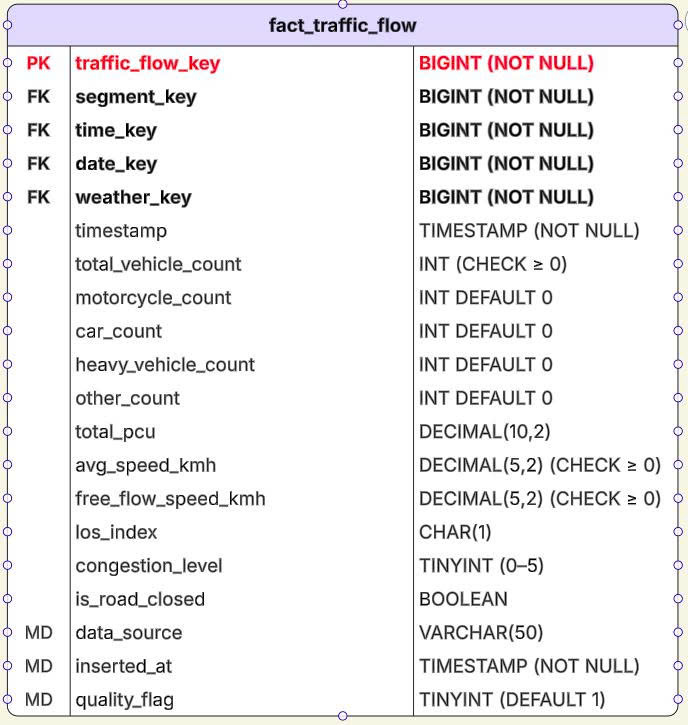
\includegraphics[width=1.0\textwidth]{Images/Picture6}
    \vspace{6mm}
    \caption{Bảng fact\_travel\_flow}
\end{figure}

\begin{figure}[H]
    \centering
   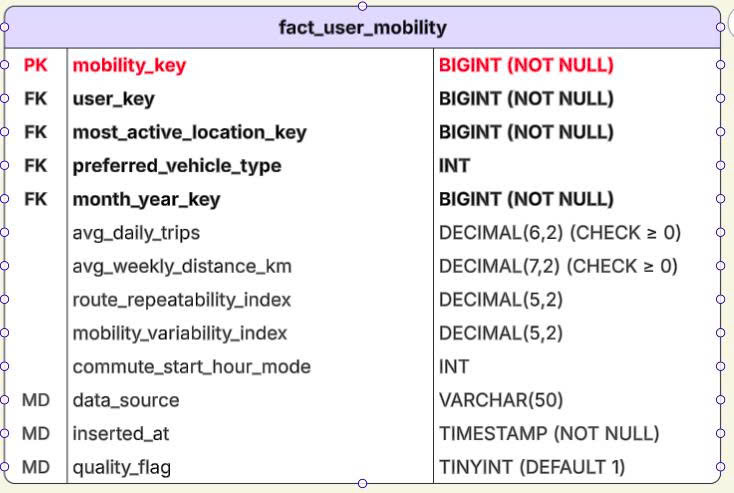
\includegraphics[width=1.0\textwidth]{Images/Picture7}
    \vspace{6mm}
    \caption{Bảng fact\_user\_mobility}
\end{figure}

\begin{figure}[H]
    \centering
    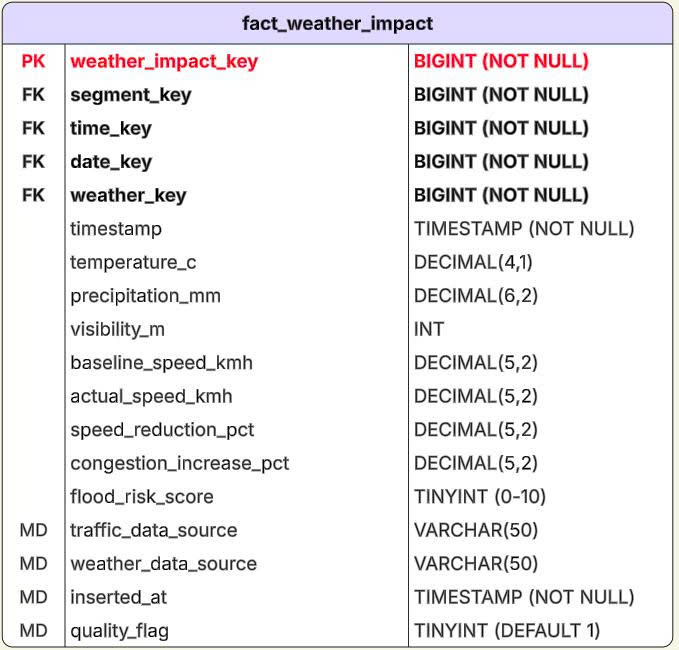
\includegraphics[width=1.0\textwidth]{Images/Picture8}
    \vspace{6mm}
    \caption{Bảng fact\_weather\_impact}
\end{figure}

\begin{figure}[H]
    \centering
   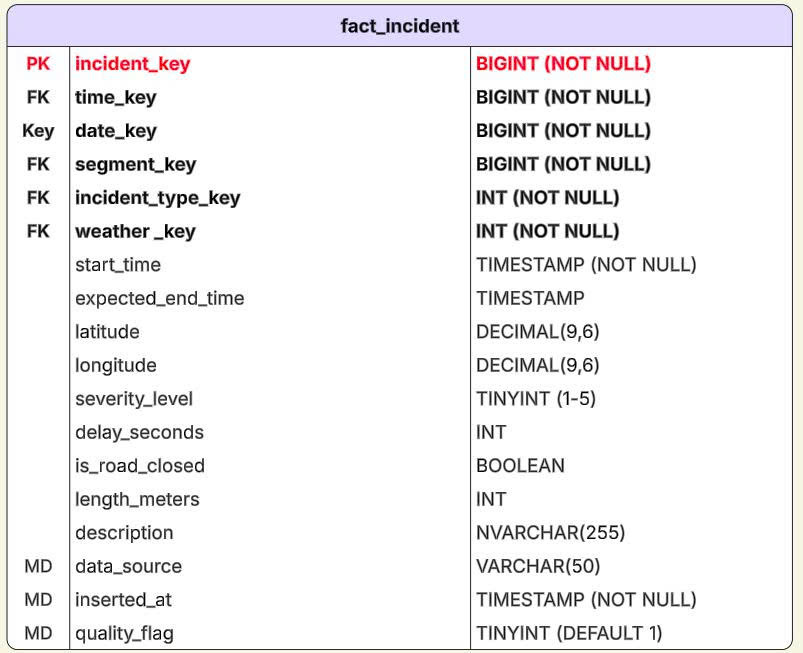
\includegraphics[width=1.0\textwidth]{Images/Picture9}
    \vspace{6mm}
    \caption{Bảng fact\_incident}
\end{figure}

\begin{figure}[H]
    \centering
    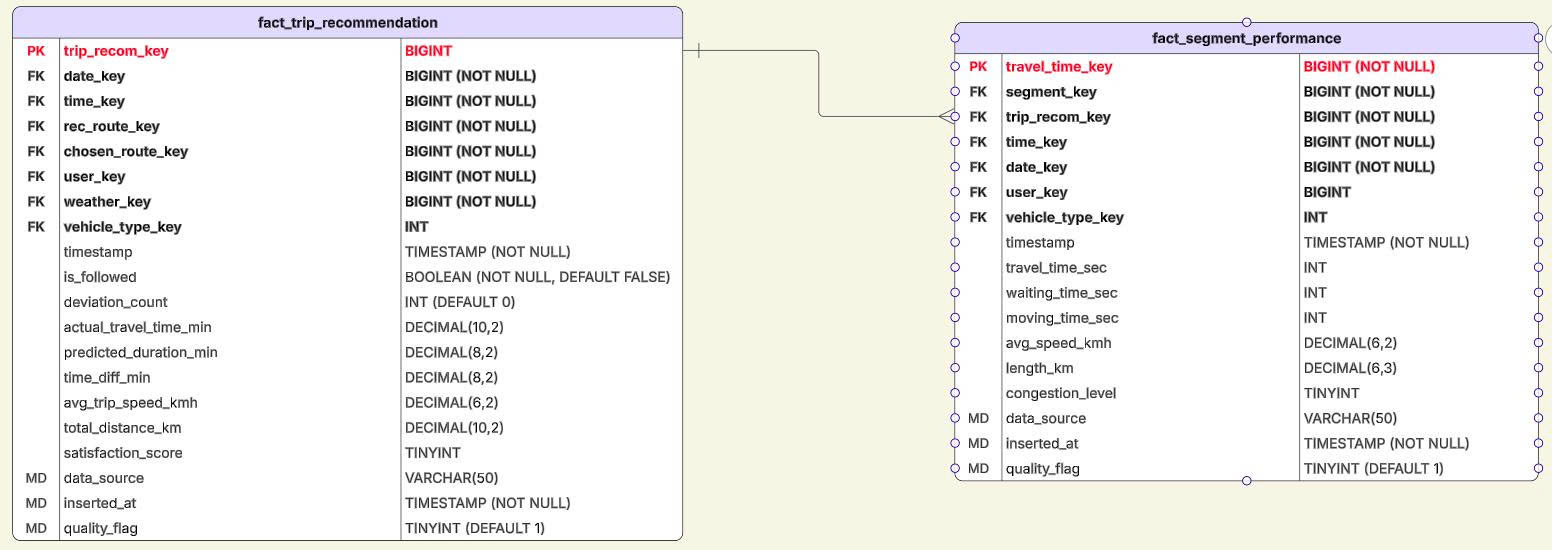
\includegraphics[width=1.0\textwidth]{Images/Picture10}
    \vspace{6mm}
    \caption{Cụm bảng fact\_trip\_recommendation và fact\_segment\_performance}
\end{figure}

\subsubsection{Bảng Dim}

\begin{figure}[H]
    \centering
    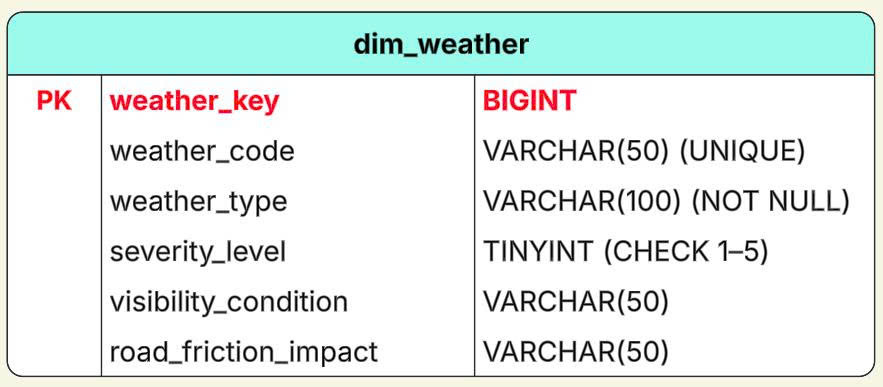
\includegraphics[width=1.0\textwidth]{Images/Picture11}
    \vspace{6mm}
    \caption{Bảng Dimension dim\_weather}
\end{figure}

\begin{figure}[H]
    \centering
    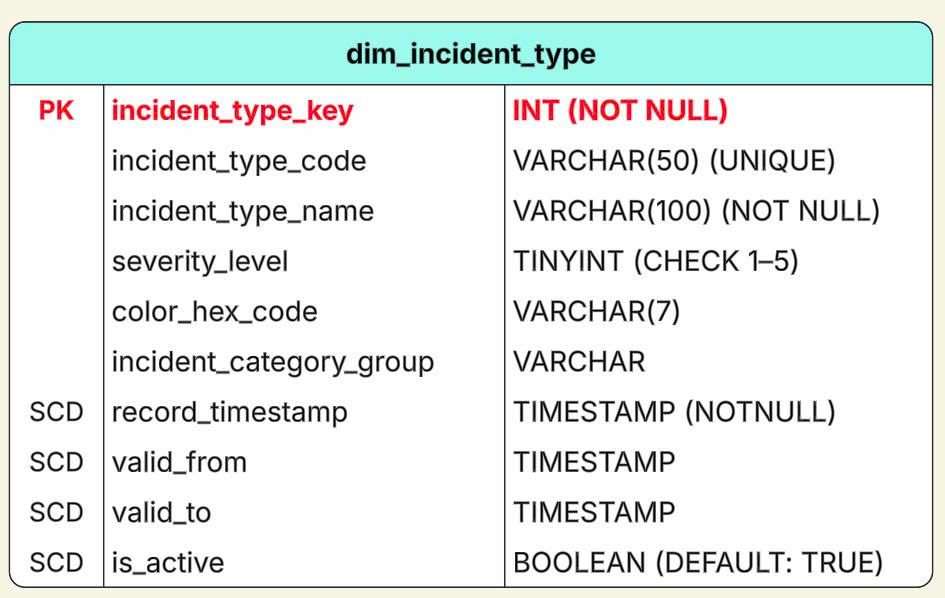
\includegraphics[width=1.0\textwidth]{Images/Picture12}
    \vspace{6mm}
    \caption{Bảng Dimension dim\_incident\_type}
\end{figure}

\begin{figure}[H]
    \centering
    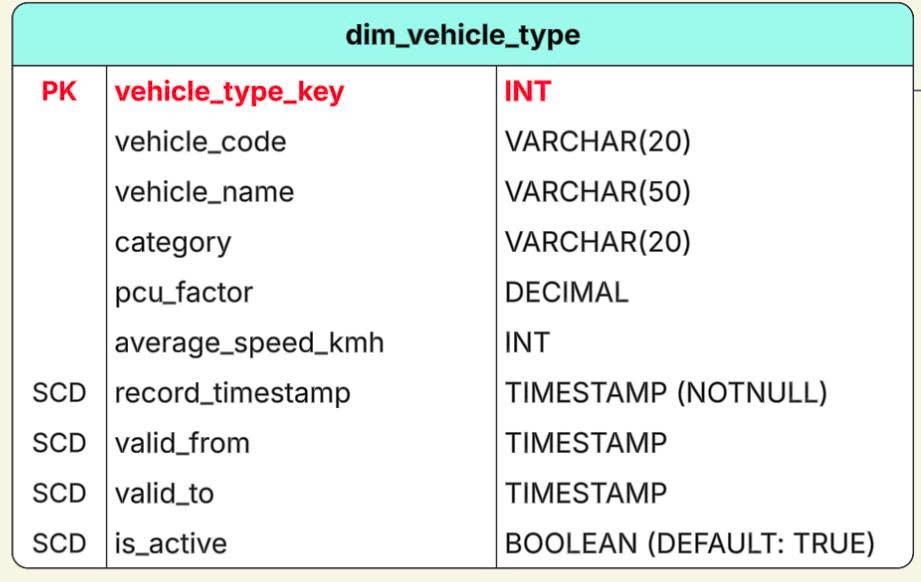
\includegraphics[width=1.0\textwidth]{Images/Picture13}
    \vspace{6mm}
    \caption{Bảng Dimension dim\_vehicle\_type}
\end{figure}

% Nhóm hình ảnh các bảng Dim liên kết (User, Time, Infrastructure)
\begin{figure}[H]
    \centering
    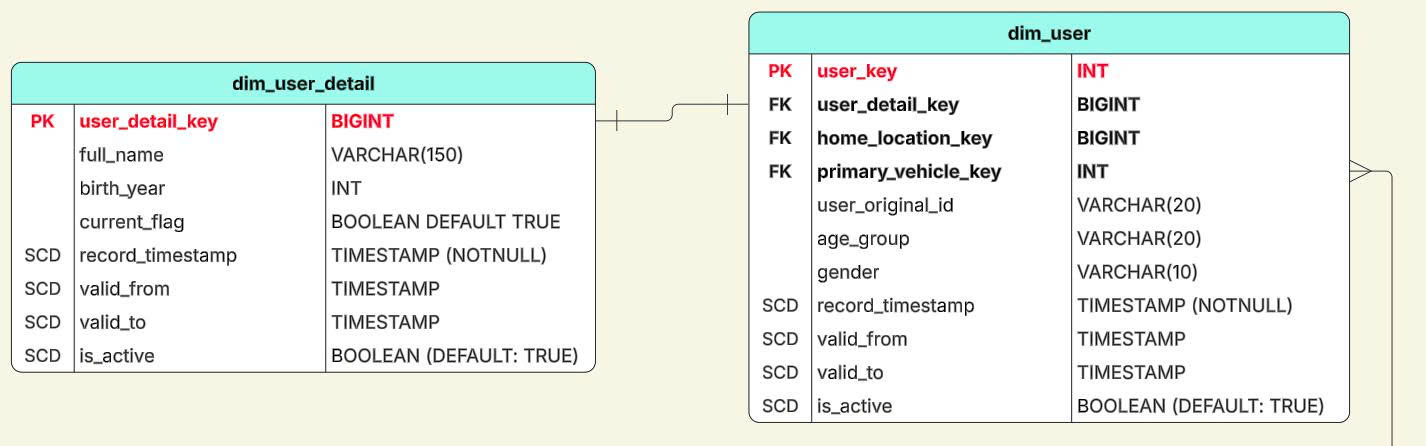
\includegraphics[width=1.0\textwidth]{Images/Picture14}
    \vspace{6mm}
    \caption{Nhóm Bảng Dimension: Người dùng}
\end{figure}

\begin{figure}[H]
    \centering
    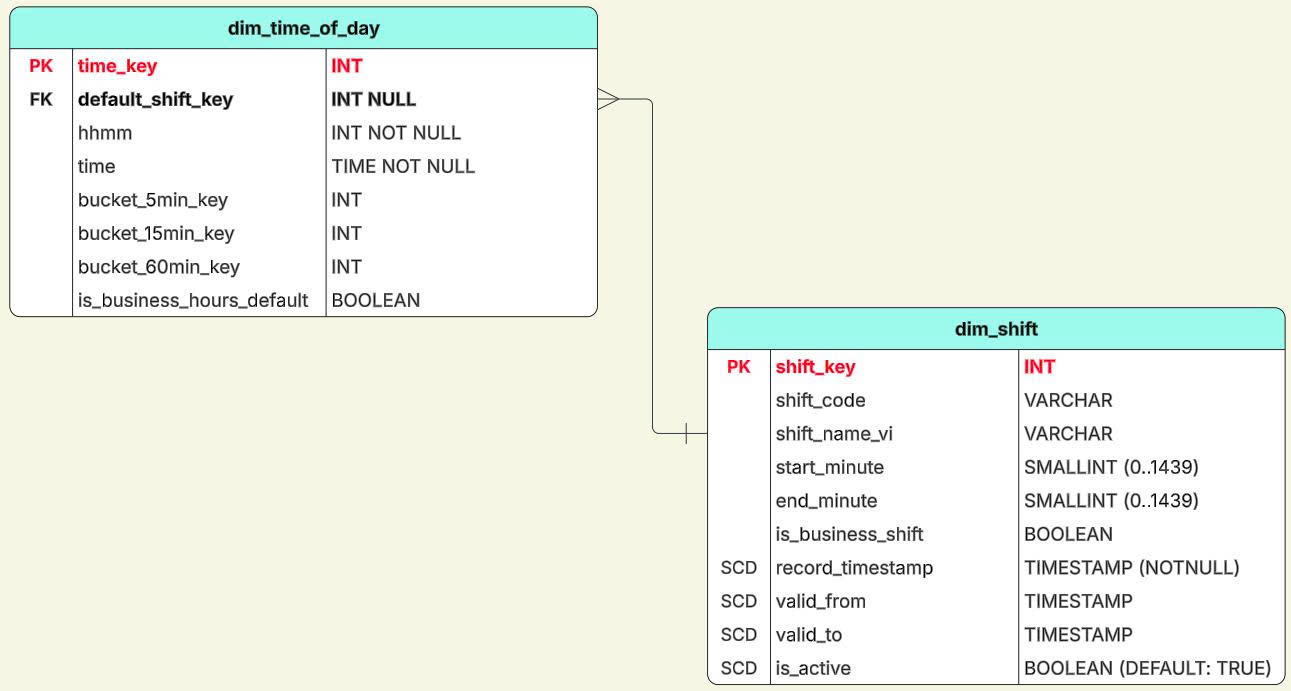
\includegraphics[width=1.0\textwidth]{Images/Picture15}
    \vspace{6mm}
    \caption{Nhóm Bảng Dimension: Thời gian (Chi tiết thời gian trong ngày)}
\end{figure}

\begin{figure}[H]
    \centering
    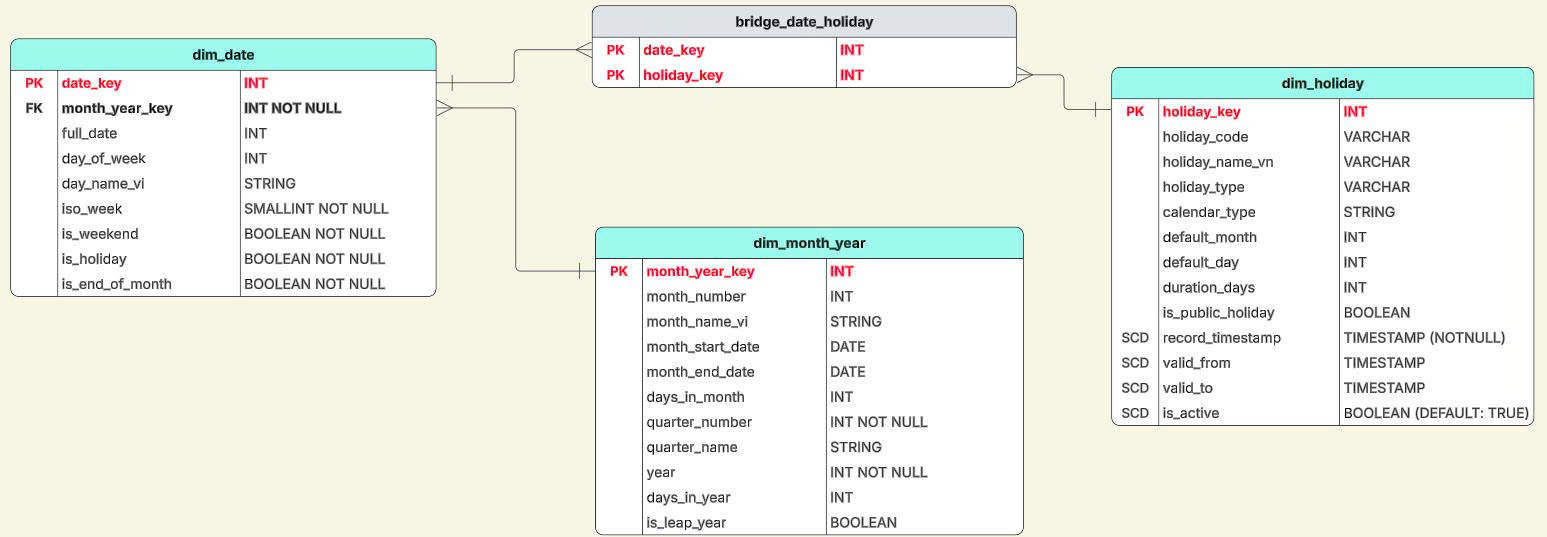
\includegraphics[width=1.0\textwidth]{Images/Picture16}
    \vspace{6mm}
    \caption{Nhóm Bảng Dimension: Thời gian (Ngày/Tháng/Năm)}
\end{figure}

\begin{figure}[H]
    \centering
    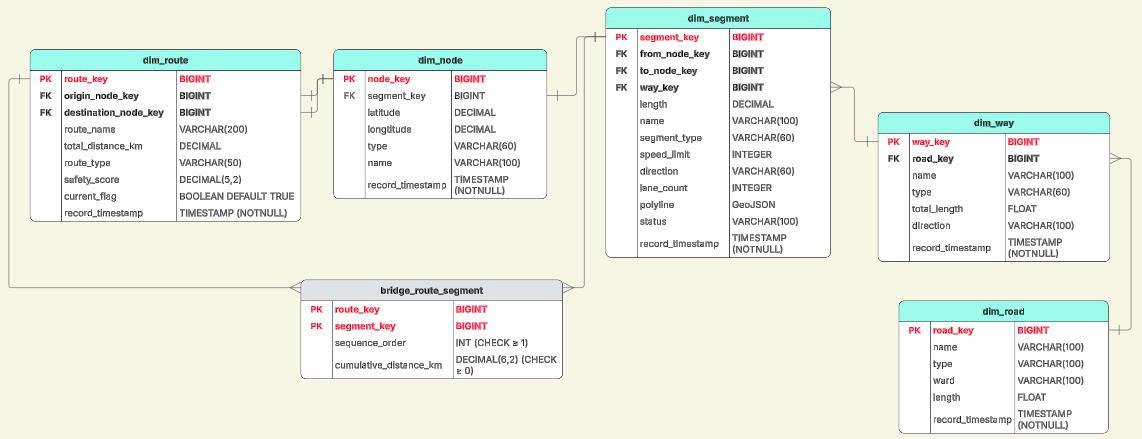
\includegraphics[width=1.0\textwidth]{Images/Picture17}
    \vspace{6mm}
    \caption{Nhóm Bảng Dimension: Hạ tầng giao thông}
\end{figure}

\subsection{Thiết kế và triển khai quy trình ETL}
\subsubsection{Quản lý ngân sách gọi API và tính bền vững}
Với nhịp độ thu thập dữ liệu dày đặc (mỗi 15 phút/lần), việc cạn kiệt hạn mức gọi API (API Quota Limit) là một rủi ro kiến trúc lớn. Hệ thống giải quyết bài toán này thông qua module quản lý TomTomKeyPool nội bộ.


Mô hình này hoạt động dựa trên cơ chế xoay vòng (Round-Robin) kết hợp với nhận thức về trạng thái (State-Aware). Thay vì sử dụng một API Key tĩnh, hệ thống duy trì một danh sách các khóa và thuật toán sẽ luôn ưu tiên cấp phát khóa có số lượt sử dụng trong ngày (usage count) thấp nhất, miễn là khóa đó chưa đạt đến daily\_limit. Đột phá hơn, hệ thống triển khai mô hình Circuit Breaker (Ngắt mạch): ngay khi API đích trả về mã lỗi 403 (Forbidden/Quota Exceeded), khóa đó ngay lập tức bị cách ly (marked as blocked) và luồng dữ liệu tự động chuyển sang khóa kế tiếp mà không làm gián đoạn tiến trình (graceful degradation).


\subsubsection{Tính lũy đẳng (Idempotency) và cơ chế xử lý xung đột dữ liệu}
Tính lũy đẳng (Idempotency) là nguyên tắc tối thượng của kiến trúc Data Warehouse được áp dụng trong dự án này. Một tác vụ ETL lũy đẳng đảm bảo rằng việc thực thi nó một hay nhiều lần vẫn tạo ra cùng một trạng thái trong cơ sở dữ liệu, không sinh ra bản ghi trùng lặp (duplicates).


Để hiện thực hóa điều này, hệ thống áp dụng cơ chế UPSERT (sử dụng cú pháp INSERT ... ON CONFLICT DO UPDATE của PostgreSQL) làm tiêu chuẩn ghi dữ liệu duy nhất trong BaseLoader. Khi chèn một lô dữ liệu (batch) vào các bảng như fact\_traffic\_flow, hệ thống sẽ dựa trên các khóa xung đột cốt lõi (ví dụ: traffic\_flow\_key, date\_key).


Nếu chưa tồn tại, hệ thống thực hiện thao tác tạo mới (INSERT).


Nếu đã tồn tại, hệ thống thực hiện cập nhật (UPDATE) các trường giá trị dẫn xuất (như current\_speed\_kmh, los\_level, congestion\_level) để đè lên dữ liệu cũ bằng dữ liệu mới nhất.


Đặc tính này là "chìa khóa" cho môi trường vận hành tự động. Khi luồng xử lý ngầm (daemon) bị khởi động lại, hay khi mạng bị lỗi gây ra các lượt chạy bù (retry), hệ thống không yêu cầu bất kỳ sự can thiệp dọn dẹp thủ công nào từ kỹ sư dữ liệu, bảo toàn tính chính xác tuyệt đối của các hệ thống Dashboard và Machine Learning downstream.


\subsubsection{Cụ thể hóa trong các Pipeline nghiệp vụ}
Tính linh hoạt của framework cốt lõi được chứng minh qua việc triển khai các pipeline con:


Traffic Pipeline: Ứng dụng BaseTransformer để cô lập logic toán học giao thông, tính toán chỉ số mức độ phục vụ (LOS) và sử dụng hàm BPR (Bureau of Public Roads) để ước lượng số lượng xe tiêu chuẩn (pcu\_volume). Logic này hoàn toàn độc lập với việc kết nối CSDL.


Incident Pipeline: Do bản chất dữ liệu là không gian (spatial), pipeline này tích hợp sâu với toán tử tìm kiếm gần nhất <-> của PostGIS và các hàm như ST\_GeomFromText để xử lý hệ tọa độ địa lý, nạp chính xác các sự cố vào bảng fact\_incident với kiểu dữ liệu geometry(Point,4326).


\subsubsection{Kiến trúc hệ thống và điều phối}
\subsubsubsection{Sơ đồ kiến trúc:}
\begin{center}
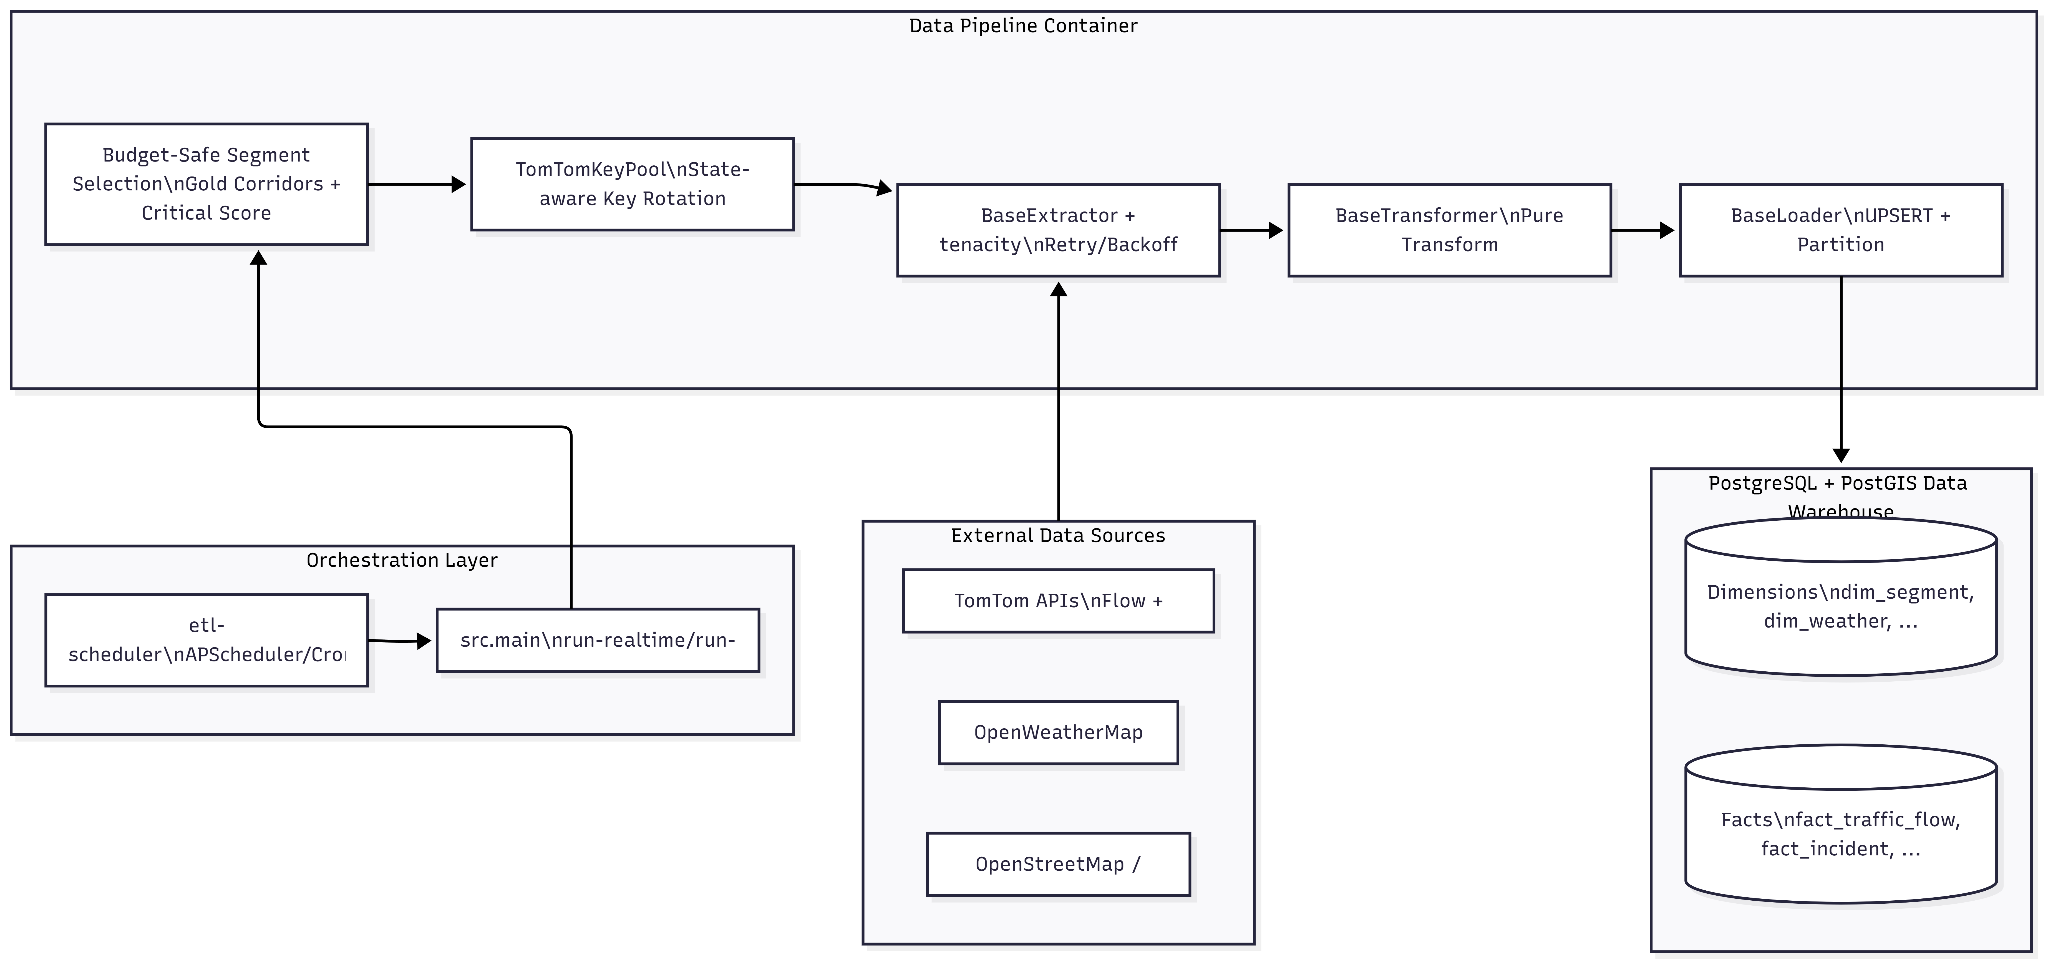
\includegraphics[width=0.85\linewidth]{Images/image17.png}
\end{center}

Hình 1: Sơ đồ kiến trúc tổng thể của hệ thống Data Pipeline trong môi trường container hóa.


Sơ đồ Hình 1 minh họa bức tranh toàn cảnh về kiến trúc hệ thống Data Pipeline, được thiết kế theo mô hình phân tán và cô lập môi trường thông qua Docker Container. Kiến trúc được chia thành 4 phân hệ logic hoạt động độc lập, tuân thủ chặt chẽ nguyên lý "Separation of Concerns" (Tách biệt mối quan tâm):


Phân hệ Nguồn dữ liệu ngoại vi (External Data Sources): Nơi cung cấp dữ liệu thô, bao gồm dữ liệu chuỗi thời gian (TomTom Flow, OpenWeatherMap) và dữ liệu không gian tĩnh (OpenStreetMap).


Phân hệ Điều phối (Orchestration Layer): Đóng vai trò là "nhịp tim" của hệ thống. Thay vì tích hợp trực tiếp cronjob vào mã nguồn ETL, hệ thống sử dụng một tiến trình lập lịch độc lập (\texttt{etl-scheduler}), tiến trình này sẽ gọi lệnh thực thi (\texttt{src.main}) theo chu kỳ chính xác. Thiết kế này giúp tách biệt logic lập lịch khỏi logic xử lý dữ liệu.


Phân hệ Xử lý Dữ liệu (Data Pipeline Container): Đây là lõi xử lý (Core Engine) của hệ thống. Luồng dữ liệu đi qua một chuỗi các trạm kiểm soát nghiêm ngặt:


Bắt đầu từ Budget-Safe Segment Selection để giới hạn phạm vi quét dựa trên ngân sách tài nguyên (Gold Corridors và Critical Score).


Tiếp tục qua TomTomKeyPool để cấp phát khóa API theo thuật toán cân bằng tải nhận thức trạng thái (State-aware Key Rotation).


Lớp BaseExtractor thực hiện gọi API với cơ chế tự động phục hồi (Retry/Backoff) nhờ thư viện \texttt{tenacity}.


Dữ liệu thô sau đó được đưa qua BaseTransformer (hoạt động dưới dạng Pure Functions) để biến đổi các chỉ số giao thông.


Cuối cùng, BaseLoader đóng gói dữ liệu để chuẩn bị ghi vào kho.


Phân hệ Lưu trữ (Data Warehouse): Cơ sở dữ liệu PostgreSQL tích hợp PostGIS tiếp nhận dữ liệu từ Loader thông qua cơ chế UPSERT để đảm bảo tính lũy đẳng (Idempotency), lưu trữ phân tách rõ ràng giữa các bảng chiều (Dimensions) và bảng sự kiện (Facts)


\subsubsubsection{Luồng thực thi tuần tự của chu kỳ ETL (Sequence Flow).}
\begin{center}
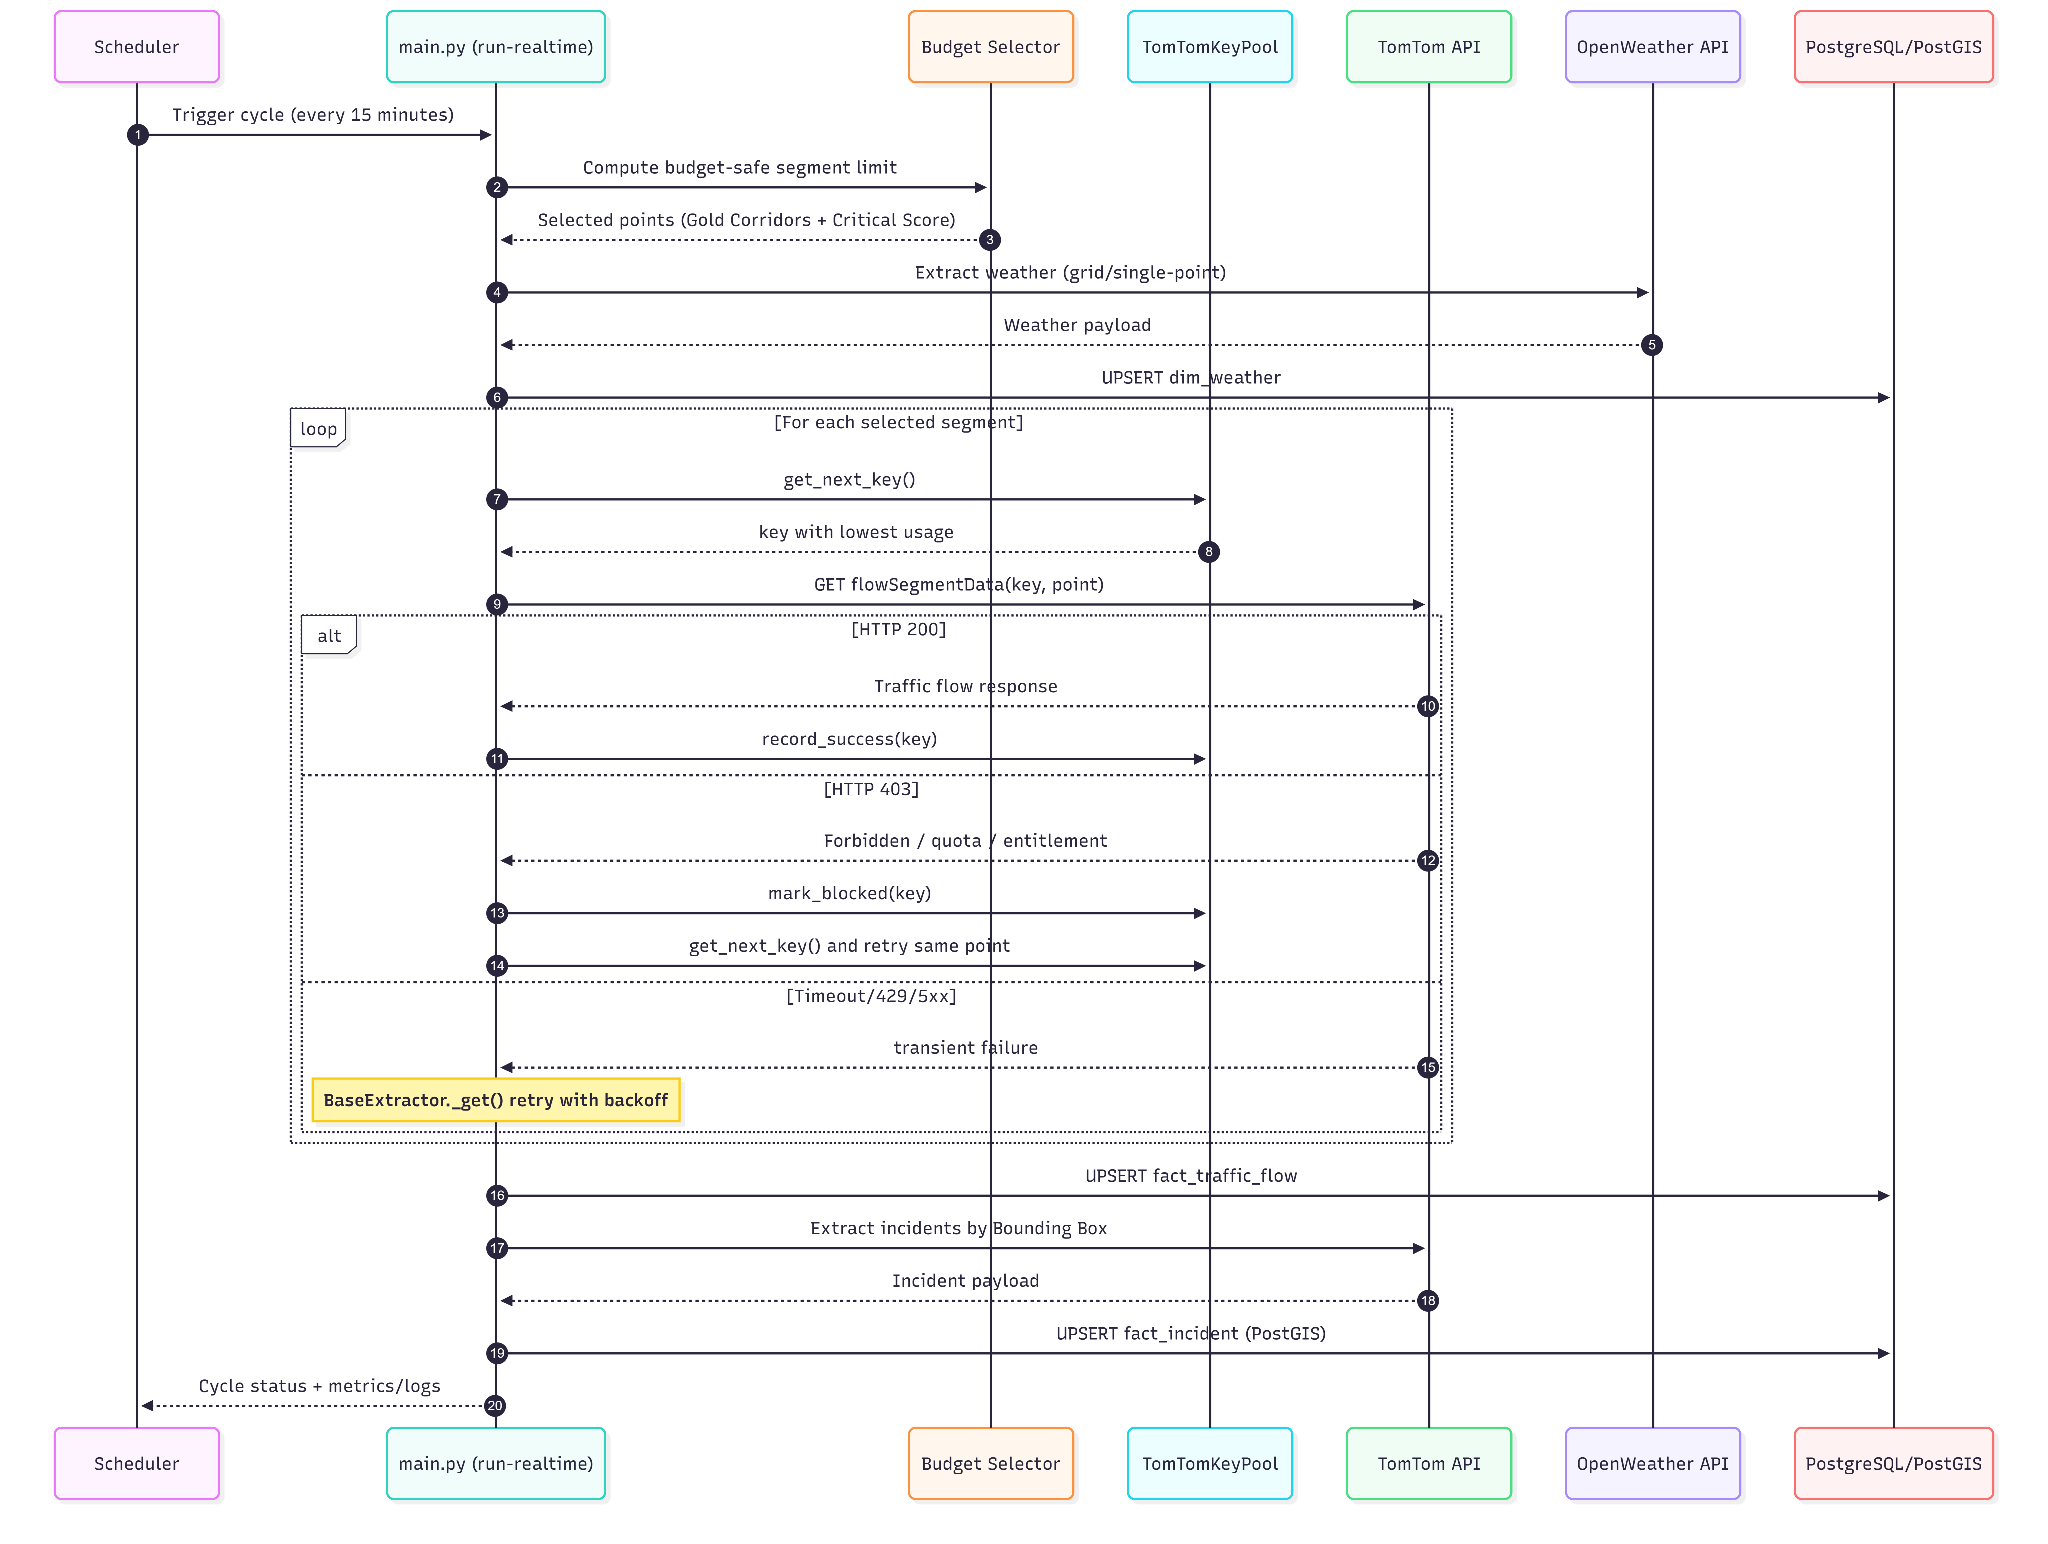
\includegraphics[width=0.85\linewidth]{Images/image7.png}
\end{center}

Sơ đồ Hình 2 mô tả chi tiết tương tác thời gian thực giữa các thực thể hệ thống trong một cửa sổ thực thi (ETL Window) kéo dài 15 phút. Chu trình này được thiết kế với độ chịu lỗi (fault-tolerance) cao, chia thành 3 giai đoạn chính:


Giai đoạn 1: Khởi tạo và Đánh giá Tài nguyên (Bước 1 - 6):


    Bộ lập lịch (Scheduler) đánh thức hệ thống. Ngay lập tức, luồng điều phối không gọi API ồ ạt mà giao tiếp với \texttt{Budget Selector} để tính toán hạn mức truy vấn an toàn. Dựa trên ngân sách này, hệ thống trích xuất danh sách các đoạn đường ưu tiên. Đồng thời, dữ liệu thời tiết (Weather) được thu thập và UPSERT ngay vào cơ sở dữ liệu làm dữ liệu ngữ cảnh (Contextual Data) cho chu kỳ hiện tại.


Giai đoạn 2: Vòng lặp Thu thập Cốt lõi và Cơ chế Chịu lỗi (Bước 7 - 15):


    Hệ thống lặp qua từng đoạn đường đã được chọn lọc. Tại mỗi vòng lặp, một cơ chế bảo vệ kép (Dual-Protection) được kích hoạt:


Bảo vệ Quota (Circuit Breaker): Trước khi gọi TomTom API, hệ thống xin cấp phát khóa từ \texttt{TomTomKeyPool}. Nếu API trả về mã lỗi \texttt{HTTP 200}, hệ thống ghi nhận thành công. Nếu API trả về \texttt{HTTP 403} (Quota/Entitlement Error), hệ thống lập tức "ngắt mạch" (mark\_blocked) khóa đó, cấp phát khóa mới và thử lại (Failover) ngay tại tọa độ đó, đảm bảo luồng không bị gãy.


Bảo vệ Mạng (Exponential Backoff): Trong trường hợp API trả về các lỗi mạng tạm thời (Timeout, 429, 5xx), lớp \texttt{BaseExtractor} tự động giam (hold) tiến trình và thử lại với độ trễ tăng dần, hấp thụ các cú sốc mạng ngắn hạn.


Giai đoạn 3: Hậu xử lý và Ghi nhận Lũy đẳng (Bước 16 - 20):


    Sau khi vòng lặp hoàn tất, một tập dữ liệu sạch hoàn chỉnh được đẩy vào bảng \texttt{fact\_traffic\_flow} qua lệnh UPSERT. Cùng lúc, dữ liệu sự cố (Incidents) được thu thập theo dạng Bounding Box, xử lý không gian (PostGIS) và UPSERT vào \texttt{fact\_incident}. Tiến trình kết thúc bằng việc trả về trạng thái (status) cho bộ điều phối, khép lại một chu kỳ toàn vẹn và không tạo ra tác dụng phụ (side-effects) cho hệ thống.


\subsubsubsection{Triển khai cấp độ điều phối}
Để đảm bảo tính độc lập với môi trường chạy thực tế, toàn bộ kiến trúc ETL được đóng gói container hóa (Containerization) thông qua nền tảng Docker. Việc này cô lập các thư viện hệ thống phức tạp (đặc biệt là GDAL/PROJ phục vụ phân tích GIS) khỏi hệ điều hành máy chủ Azure VM.


Ở cấp độ điều phối, kiến trúc triển khai loại bỏ việc phụ thuộc vào cronjob truyền thống để thay thế bằng mô hình Daemon-driven Execution (Thực thi bằng tiến trình ngầm) thông qua module run-cycle-daemon trong main.py. Module này giám sát chặt chẽ chu kỳ thời gian thực, có khả năng tự động tính toán lại độ trễ (drift correction), kiểm soát khung giờ vàng giao thông (ETL Window) và thực thi chiến lược định tuyến ưu tiên (Critical Segment Selection). Điều này không chỉ tối ưu hóa khối lượng API được gọi mà còn biến pipeline thành một khối dịch vụ (service block) tự chủ, mạnh mẽ và ổn định lâu dài trên đám mây.


\subsubsection{Thu thập dữ liệu}
\subsubsubsection{Ràng buộc tài nguyên trong Data Ingestion}
Trong các hệ thống Data Warehouse hiện đại, giai đoạn thu thập dữ liệu (Data Ingestion) thường phải đối mặt với bài toán tối ưu hóa đa mục tiêu: Tốc độ (Velocity), Khối lượng (Volume) và Giá trị (Value). Đối với dự án Traffic IoC, chiến lược Extraction không được thiết kế theo tư duy "quét toàn bộ không gian" (Brute-force/Full-scan) ở mỗi chu kỳ 15 phút. Nguyên nhân cốt lõi xuất phát từ hai ràng buộc kỹ thuật khắt khe:


Giới hạn về hạn mức gọi API (Quota Limits) từ các nhà cung cấp bên thứ ba như TomTom và OpenWeatherMap


Yêu cầu đảm bảo tính liên tục của luồng Data Pipeline (thực thi 61 chu kỳ mỗi ngày từ 6h sáng đến 21h tối) mà không được phép xảy ra hiện tượng cạn kiệt tài nguyên (Resource Exhaustion).


Để giải quyết bài toán này, hệ thống áp dụng tư duy Budget-Aware, Priority-Driven, and Fault-Tolerant Ingestion (Thu thập dữ liệu chịu lỗi, định hướng ưu tiên và nhận thức ngân sách). Đây là một chiến lược tối ưu hóa kiến trúc, giúp cân bằng giữa độ phủ không gian của dữ liệu, chi phí vận hành API và tính ổn định của toàn bộ chu trình ETL.


\subsubsubsection{Xây dựng kế hoạch "Budget-Safe Realtime" và lấy mẫu có trọng số}
\textbf{Phân bổ ngân sách gọi API động (Dynamic Budget Allocation)}\\
Để ngăn chặn luồng realtime bào mòn hạn mức API quá nhanh, hệ thống triển khai cơ chế tự động tính toán "ngưỡng an toàn" (budget limit) cho từng chu kỳ 15 phút. Việc tính toán này được tham số hóa hoàn toàn thông qua các biến môi trường, loại bỏ các giá trị hard-code cứng nhắc. Công thức phân bổ ngân sách lý thuyết được triển khai như sau:


raw = max(1, n\_keys * daily\_limit // cycles - reserve)


Trong đó:


n\_keys: Tổng số lượng API Keys đang khả dụng trong Pool.


daily\_limit: Giới hạn truy vấn tối đa của một Key trong 24 giờ (mặc định 2500).


cycles: Tổng số lần kích hoạt pipeline trong ngày (mặc định 61 chu kỳ).


reserve và headroom: Vùng đệm an toàn để dự phòng cho các truy vấn phát sinh ngoài luồng giao thông (ví dụ: truy vấn sự cố - incidents).


Ý nghĩa kiến trúc của cơ chế này là biến một tiến trình batch-micro tĩnh thành một hệ thống nhận thức tài nguyên (Resource-aware System). Bất kể số lượng Key bị hao hụt hay bị khóa trong ngày, hệ thống tự động co giãn (scale down) số lượng đoạn đường cần quét, bảo vệ tính liên tục của pipeline trước rủi ro sụp đổ hệ thống (System Crash) do chạm ngưỡng giới hạn.


\subsubsubsection{Kỹ thuật lựa chọn ưu tiên: Gold Corridors và Critical Score}
Khi ngân sách truy vấn (budget) trong một chu kỳ nhỏ hơn tổng số đoạn đường thực tế trong bảng dim\_segment, hệ thống phải thực hiện thao tác cắt tỉa (pruning). Luồng định tuyến (Routing logic) sử dụng thuật toán Priority-Constrained Sampling (Lấy mẫu có ràng buộc ưu tiên).


Hệ thống đánh giá các ứng viên dựa trên hai tiêu chí định lượng:


Mức độ quan trọng của hành lang (Corridor Importance Level): Chỉ tập trung quét các đoạn đường thuộc nhóm "Gold Corridors" (Hành lang vàng) - các trục giao thông huyết mạch đã được định nghĩa trong bảng dim\_corridor.


Điểm tới hạn (Critical Score): Hệ thống ưu tiên các đoạn đường có lịch sử tắc nghẽn hoặc rủi ro cao (dựa trên dữ liệu đã phân tích ở các chu kỳ trước).


Thuật toán phân bổ ngân sách hoạt động theo phương pháp tiếp cận tham lam (Greedy Approach) qua hai vòng lặp (Pass 1 \& Pass 2), đảm bảo bao phủ tối thiểu toàn bộ các hành lang trọng điểm trước khi dùng ngân sách dư thừa để quét các đoạn đường ưu tiên cao. Về mặt học thuật, chiến lược này hy sinh độ phủ không gian tuyệt đối (Absolute Spatial Coverage) để tối ưu hóa giá trị thông tin thu về (Information Value Maximization), cung cấp một tập dữ liệu đầu vào cực kỳ chất lượng cho bảng fact\_traffic\_flow mà không gây lãng phí tài nguyên mạng.


\subsubsection{Cơ chế quản lý khóa API động và cân bằng tải}
\subsubsubsection{Nhận thức trạng thái}
Với nhịp độ 15 phút/lần, việc dựa vào một API key duy nhất tạo ra một điểm nghẽn cổ chai (Single Point of Failure - SPOF) nghiêm trọng. Module TomTomKeyPool giải quyết triệt để vấn đề này bằng cách thiết lập một cơ chế Cân bằng tải vòng lặp (Round-Robin Load Balancing) có lưu trữ trạng thái.


Hệ thống liên tục theo dõi biến usage (số lần đã gọi) của từng Key. Mỗi khi cần phát lệnh HTTP mới, thuật toán không chọn ngẫu nhiên mà luôn cấp phát Key đang có mức sử dụng thấp nhất và chưa đạt giới hạn daily\_limit.


\subsubsubsection{Mẫu thiết kế Circuit Breaker và Failover tự động}
Đột phá của kiến trúc nằm ở khả năng tự động xử lý khi một Key bị từ chối dịch vụ (HTTP 403 Forbidden hoặc Quota Exceeded). Hệ thống áp dụng mẫu thiết kế Circuit Breaker (Ngắt mạch): ngay khi phát hiện chuỗi phản hồi 403, Key đó lập tức bị dán nhãn blocked (cách ly) cho đến hết ngày.


Đồng thời, cơ chế Graceful Failover (Chuyển đổi dự phòng êm ái) được kích hoạt. Lớp Extractor tự động nạp Key khả dụng tiếp theo từ Pool và thử lại chính xác tọa độ bị lỗi trước đó mà không làm đứt gãy luồng thực thi vòng lặp hiện tại. Trạng thái của Pool (usage và blocked) được lưu trữ liên tục (persist) vào file JSON tại /app/cache/tomtom\_key\_pool\_state.json. Điều này đảm bảo tính toàn vẹn của trạng thái API (Statefulness) ngay cả khi môi trường Docker Container bị khởi động lại (restart), ngăn chặn việc tái sử dụng nhầm các Key đã cạn kiệt ngân sách.


\subsubsection{Sức bền mạng và khả năng chịu lỗi}
\subsubsubsection{Cơ chế Retry with Exponential Backoff}
Trong môi trường điện toán đám mây phân tán, các lỗi mạng như rớt gói tin (packet loss), Timeout, hay HTTP 502/503/504 (Bad Gateway) là những "lỗi hiển nhiên" (transient faults) luôn xảy ra. Tầng BaseExtractor chặn đứng sự lan truyền của các lỗi này bằng cách sử dụng thư viện tenacity để tự động hóa chiến lược Retry with Backoff.


Mọi truy vấn HTTP đều được bao bọc (wrapped) trong một bộ nguyên tắc chặt chẽ: thử lại tối đa 3 lần, khoảng cách chờ (wait interval) là 2 giây. Chiến lược này có khả năng hấp thụ (absorb) các cú sốc mạng ngắn hạn, giúp tỷ lệ thành công của các chu kỳ thu thập tiệm cận mức tuyệt đối.


\subsubsubsection{Xử lý phân cực: lỗi tạm thời với lỗi hệ thống}
Về mặt nguyên lý hệ thống, BaseExtractor phân biệt cực kỳ rạch ròi giữa Lỗi Tạm thời (Transient Errors - mã HTTP 429, 5xx) và Lỗi Không thể phục hồi (Non-recoverable Errors - mã HTTP 400, 401, 404).


Các mã lỗi tạm thời được đẩy vào vòng lặp Retry để chờ mạng phục hồi.


Các mã lỗi 4xx (ngoại trừ 429) phản ánh lỗi sai cú pháp hệ tọa độ, cấu hình URL sai hoặc thiếu quyền truy cập (Unauthorized). Hệ thống sẽ lập tức ném ra ngoại lệ DataExtractionError để cắt đứt ngay truy vấn đó thay vì Retry vô nghĩa, tránh việc rơi vào vòng lặp vô tận (Infinite Loop) làm treo (hang) tiến trình ETL hiện hành.


\subsubsection{Đa dạng hóa nguồn thu thập và xử lý bất đồng bộ}
\subsubsubsection{Thu thập dữ liệu tĩnh (Topology) vs. Động (Time-series)}
Dự án thiết lập hai nhịp độ thu thập hoàn toàn tách biệt dựa trên đặc tính chu kỳ của dữ liệu:


Mạng lưới không gian tĩnh (Spatial Network Topology): Sử dụng thư viện osmnx để bóc tách dữ liệu từ OpenStreetMap (OSM). Do tính chất ít biến động của hạ tầng cầu đường, luồng này hoạt động theo cơ chế Batch Processing (chỉ chạy khi khởi tạo hệ thống hoặc có yêu cầu refresh hạ tầng). Dữ liệu sau đó được định tuyến chuẩn xác vào các bảng Dimensions cốt lõi: dim\_node, dim\_road, dim\_way, và dim\_segment.


Dữ liệu sự kiện động (Dynamic Time-series Facts): Luồng TomTom Traffic Flow và TomTom Incidents đại diện cho dữ liệu luồng (Streaming/Micro-batch). Chúng thay đổi liên tục từng phút, bắt buộc phải sử dụng chiến lược Real-time Extract với giới hạn ngân sách chặt chẽ như đã phân tích ở trên.


\subsubsection{Mở rộng kích thước lưới cho dữ liệu bổ trợ}
Đối với luồng OpenWeatherMap bổ trợ cho bảng dim\_weather, thay vì gọi API cho từng tọa độ đoạn đường (segment) nhỏ lẻ một cách lãng phí, kiến trúc sư dữ liệu đã thiết kế chiến lược thu thập theo dạng Lưới không gian (Grid-based Extraction). Thành phố được chia thành các ô lưới (Grid size), và thời tiết được nội suy cho toàn bộ các đoạn đường nằm trong ô lưới đó. Điều này minh chứng cho tính linh hoạt của BaseExtractor: một khung kiến trúc nhưng áp dụng được nhiều kỹ thuật tối ưu không gian khác nhau, chuẩn bị hoàn hảo cho giai đoạn Transform phức tạp phía sau.


\subsubsection{Trình tự nạp dữ liệu và ràng buộc}
\subsubsubsection{Nguyên lý ràng buộc toàn vẹn tham chiếu và cấu trúc DAG}
Trong lý thuyết thiết kế Kho dữ liệu (Data Warehouse) sử dụng mô hình Galaxy Schema, luồng thực thi ETL không thể tiến hành nạp dữ liệu song song (parallel loading) một cách tùy ý cho tất cả các bảng. Về bản chất toán học, các bảng trong cơ sở dữ liệu và các Ràng buộc Khóa ngoại (Foreign Key Constraints) tạo thành một Đồ thị có hướng không chu trình (DAG - Directed Acyclic Graph). Trong đồ thị này, các đỉnh (nodes) đại diện cho các bảng, và các cạnh có hướng (directed edges) biểu diễn quan hệ phụ thuộc từ bảng chứa khóa ngoại (Bảng con) trỏ về bảng chứa khóa chính (Bảng cha).


\begin{center}
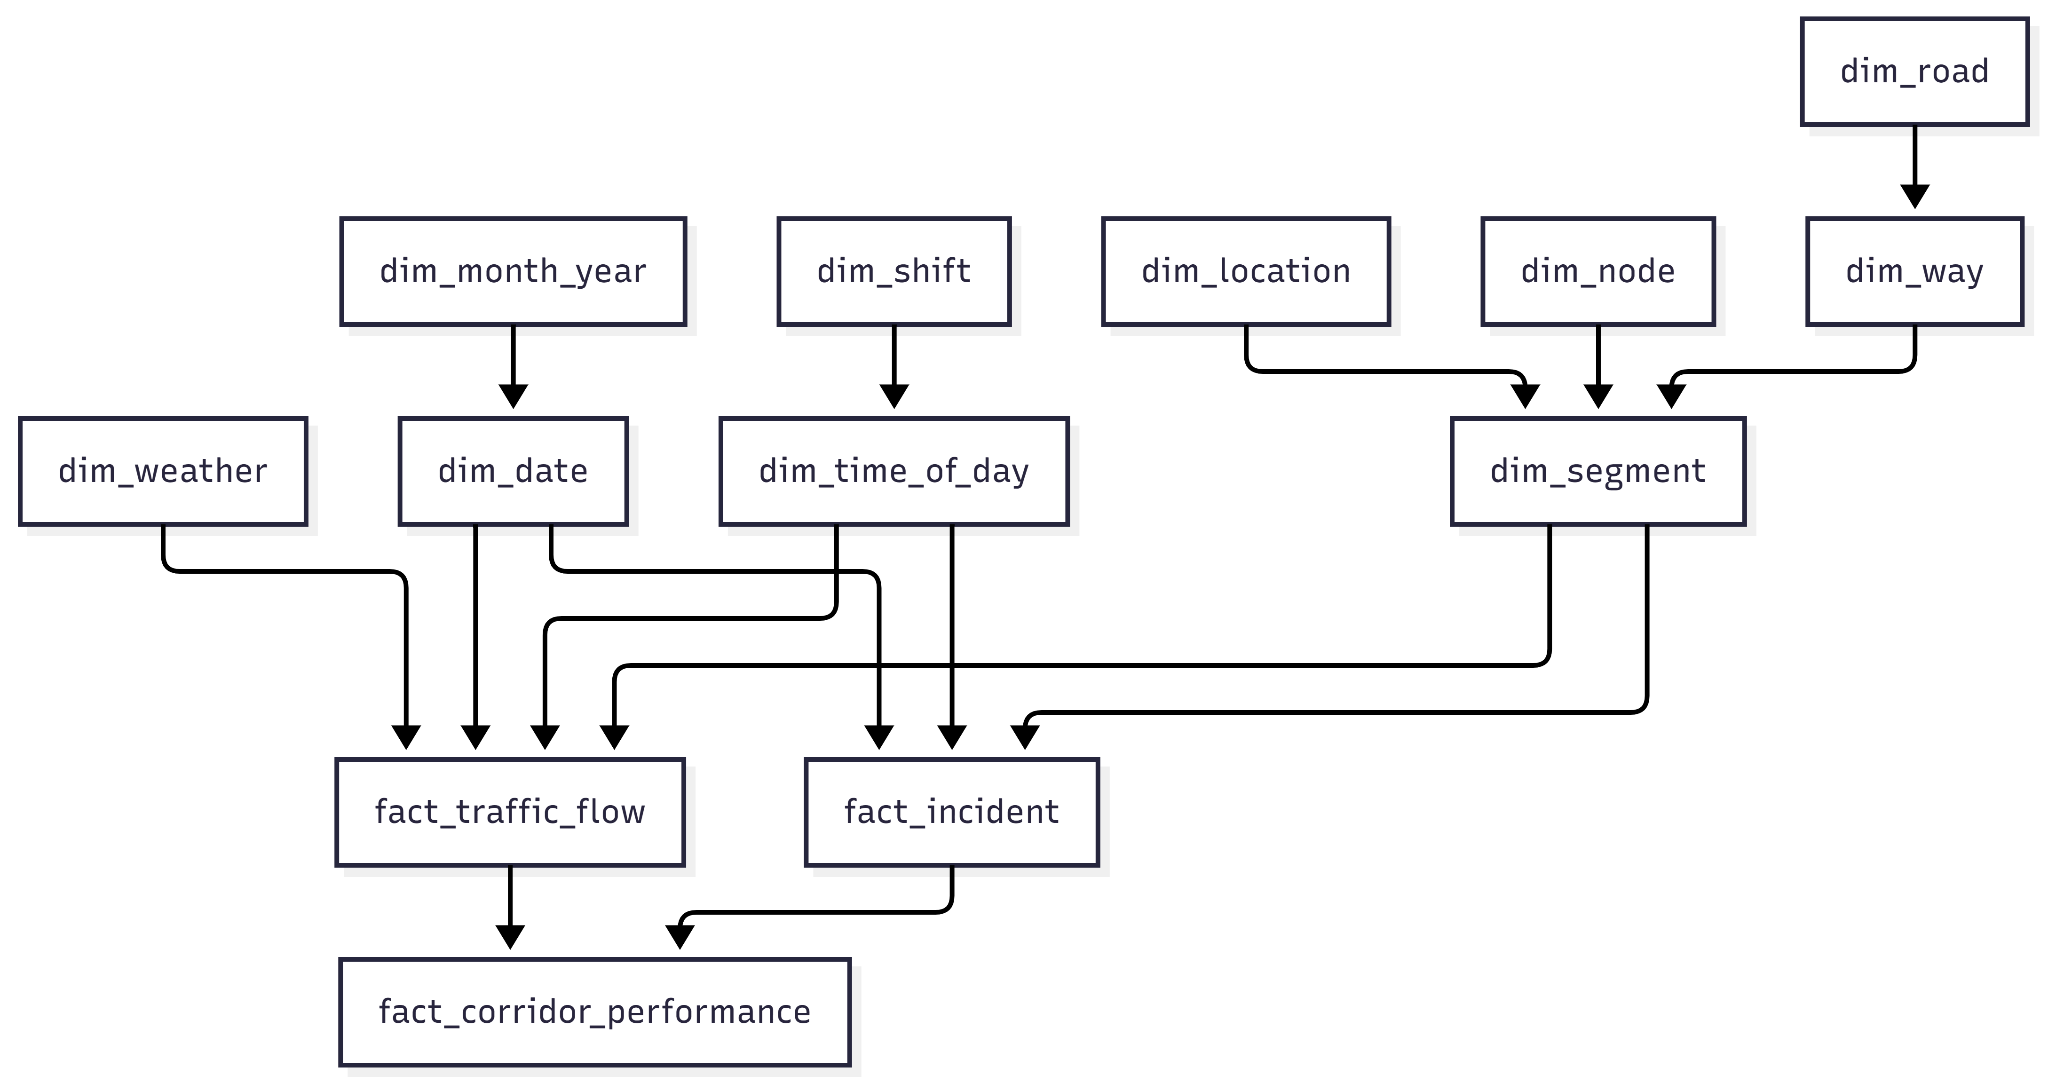
\includegraphics[width=0.85\linewidth]{Images/image3.png}
\end{center}

Để duy trì Ràng buộc Toàn vẹn Tham chiếu (Referential Integrity), chiến lược nạp dữ liệu bắt buộc phải tuân thủ thuật toán Sắp xếp Tô-pô (Topological Sort). Nếu pipeline vi phạm trình tự này (ví dụ: nạp dữ liệu luồng giao thông trước khi nạp thông tin đoạn đường), hệ quản trị PostgreSQL sẽ lập tức từ chối giao dịch (Transaction Rollback) kèm theo lỗi Foreign Key Violation. Do đó, kiến trúc Pipeline của dự án được phân rã thành 4 pha (Phases) thực thi tuần tự nghiêm ngặt.


\subsubsubsection{Pha 1: Khởi tạo dữ liệu nền tảng}
Pha đầu tiên tập trung giải quyết các đỉnh gốc (root nodes) của đồ thị DAG – đây là các bảng Chiều (Dimension Tables) không chứa khóa ngoại, hoặc chỉ chứa khóa ngoại tham chiếu lẫn nhau trong một cụm độc lập. Mục tiêu của pha này là xây dựng hệ quy chiếu về Không gian, Thời gian và Ngữ cảnh.


Hệ quy chiếu Thời gian (Temporal Dimensions): Dữ liệu được nạp theo chuỗi phụ thuộc tuyến tính: dim\_month\_year $\rightarrow$  dim\_date và dim\_shift $\rightarrow$ dim\_time\_of\_day. Đây là các bảng tĩnh, thường được nạp sẵn dữ liệu (pre-populated) cho nhiều năm, làm nền tảng phân hoạch (partitioning) cho toàn bộ Data Warehouse.

Chiều Ngữ cảnh (Contextual Dimension): Bảng dim\_weather đóng vai trò là một Slow Changing Dimension (SCD) cung cấp thông tin ngữ cảnh thời tiết. Vì thời tiết thay đổi liên tục, module thời tiết sẽ được kích hoạt nạp trước tiên trong chu kỳ 15 phút, sinh ra weather\_key để chuẩn bị gán vào các sự kiện giao thông phát sinh cùng thời điểm.


\subsubsubsection{Pha 2: Xây dựng Topology Không gian}
Pha thứ hai là trái tim của mô hình Snowflake không gian, do module osm\_pipeline.py đảm nhiệm. Khác với các hệ thống thông thường, mạng lưới đường bộ có tính phụ thuộc hình học (Geometric Dependency) cực kỳ khắt khe. Dữ liệu bắt buộc phải được nạp (UPSERT) theo trình tự giải phẫu topology:


dim\_node (Nút giao): Nạp đầu tiên, chứa tọa độ geometry(Point,4326) nguyên thủy.


dim\_road (Tuyến đường): Nạp thông tin định danh tuyến đường (tên đường, tổng chiều dài).


dim\_way (Phân đoạn OSM): Trỏ khóa ngoại road\_key về dim\_road, lưu trữ các thuộc tính thiết kế như số làn đường mặc định, giới hạn tốc độ.


dim\_segment (Đoạn đường vật lý): Là "nút hội tụ" cuối cùng của cụm không gian. Một đoạn đường thực tế được cấu thành từ một điểm đầu, một điểm cuối và thuộc về một tuyến đường. Do đó, dim\_segment bắt buộc phải nạp cuối cùng để có thể nhận đủ 3 khóa ngoại: from\_node\_key, to\_node\_key, và way\_key.


\subsubsubsection{Pha 3: Nạp dữ liệu chuỗi thời gian}
Sau khi Pha 1 và Pha 2 hoàn tất, toàn bộ hệ quy chiếu đã sẵn sàng. Lúc này, luồng thực thi thời gian thực (traffic\_pipeline.py và incident\_pipeline.py) mới được kích hoạt.


Trong thiết kế kiến trúc, các bảng fact\_traffic\_flow và fact\_incident đóng vai trò là các "Sinks" (Điểm trũng / Nút lá) của đồ thị DAG. Chúng là nơi hội tụ của mọi khóa ngoại.


Bảng fact\_traffic\_flow sẽ hấp thụ đồng thời segment\_key (từ Pha 2), date\_key, time\_key và weather\_key (từ Pha 1).


Bảng fact\_incident cũng tương tự, kết hợp thêm dữ liệu không gian geometry(Point,4326) để mô tả vị trí xảy ra sự cố.


Đặc biệt, ở Pha này, chiến lược nạp dữ liệu kết hợp trực tiếp với tính năng Table Partitioning của PostgreSQL. Hệ thống không ghi toàn bộ vào một bảng khổng lồ mà định tuyến dữ liệu vào các phân vùng theo tháng (ví dụ: fact\_traffic\_flow\_202603) dựa trên giá trị của date\_key. Điều này triệt tiêu tình trạng thắt cổ chai I/O (I/O Bottleneck) khi lưu lượng ghi vào database tăng đột biến ở các khung giờ cao điểm.


\subsubsubsection{Pha 4: Hậu xử lý và dữ liệu phái sinh}
Pha cuối cùng là các luồng phân tích theo lô (Batch Processing), tiêu biểu là pipeline hiệu suất hành lang (corridor\_pipeline.py).


Bảng fact\_corridor\_performance lưu trữ Dữ liệu Phái sinh (Derived Data). Xét về sự phụ thuộc (Data Dependency), nó không trích xuất trực tiếp từ API bên ngoài mà sử dụng kết quả truy vấn (JOIN và Aggregation) từ bảng fact\_traffic\_flow và cầu nối bridge\_corridor\_segment.


Vì tính chất này, logic điều phối (main.py) buộc phải lập lịch cho Pha 4 chạy vào cuối ngày (Nightly Batch), SAU KHI các bảng Fact ở Pha 3 đã thu thập đầy đủ và ổn định dữ liệu. Việc thiết lập quan hệ phụ thuộc thời gian (Temporal Dependency) giữa các tiến trình ETL đảm bảo các chỉ số tổng hợp (như travel\_time\_index hay corridor\_efficiency) phản ánh chính xác bức tranh giao thông của toàn bộ ngày vận hành.


\subsection{Logic Biến đổi Dữ liệu}
\subsubsection{Nguyên lý hàm thuần túy trong tầng biến đổi}
Trong kiến trúc của hệ thống Data Pipeline, pha Transform đóng vai trò là "hạt nhân tính toán" (Computational Engine). Về mặt kỹ nghệ phần mềm, toàn bộ các phép biến đổi nghiệp vụ tại lớp BaseTransformer được thiết kế tuân thủ nghiêm ngặt nguyên lý Hàm Thuần túy (Pure Functions) của Lập trình Hàm (Functional Programming).


Đặc trưng cốt lõi của kiến trúc này là sự vắng mặt hoàn toàn của các "tác dụng phụ" (side-effects). Tầng Transform không thực hiện bất kỳ giao tiếp I/O nào (không gọi API bên ngoài, không truy vấn ngược về cơ sở dữ liệu, không ghi file). Mọi tính toán từ việc ước lượng lưu lượng xe, phân loại mức độ phục vụ (LOS), đến chuẩn hóa tọa độ đều được thực hiện hoàn toàn trong bộ nhớ (in-memory). Quyết định thiết kế này mang lại ba giá trị học thuật to lớn đối với một Data Warehouse:


Tính tất định (Determinism): Đảm bảo rằng với một tập dữ liệu thô (raw payload) đầu vào, bộ chuyển đổi luôn sinh ra một và chỉ một tập dữ liệu chuẩn hóa duy nhất.


Khả năng kiểm thử cô lập (Isolated Testability): Cho phép triển khai các Unit Test bao phủ toàn bộ logic toán học mà không cần thiết lập (mock) các môi trường cơ sở dữ liệu phức tạp.


Tính tái lập (Reproducibility): Khi xảy ra sự cố cần nạp bù dữ liệu (backfill), kỹ sư dữ liệu có thể chạy lại luồng Transform một cách an toàn mà không lo ngại về trạng thái (state) hệ thống làm sai lệch kết quả.


\subsubsection{Khai phá và biến đổi động lực học dòng xe}
Dữ liệu đầu vào từ API TomTom chủ yếu là các tham số vận tốc. Nhiệm vụ của luồng traffic\_pipeline.py là sử dụng các mô hình toán học giao thông để chuyển đổi vận tốc thô thành các chỉ số mô tả bức tranh động lực học dòng xe, sau đó nạp vào bảng fact\_traffic\_flow.


\subsubsubsection{Chuỗi biến đổi chỉ số cơ bản (Traffic Index, Delay \& LOS)}
Hệ thống sử dụng các phép toán vô hướng để thiết lập các chỉ số cơ bản:


Tỷ lệ vận tốc (Speed Ratio - r): Được định nghĩa là tỷ số giữa vận tốc thực tế (v) và vận tốc thiết kế/thông thoáng ($v_f$).


\begin{center}
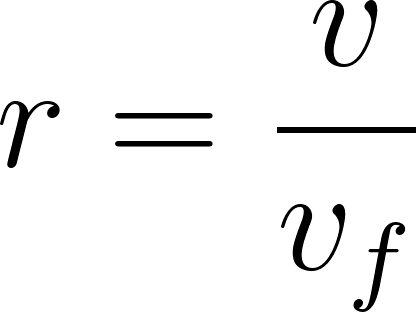
\includegraphics[width=0.1\linewidth]{Images/image6.png}
\end{center}

Chỉ số ùn tắc (Traffic Index - I): Biểu diễn mức độ suy giảm vận tốc so với điều kiện lý tưởng, được lưu vào cột traffic\_index.


\begin{center}
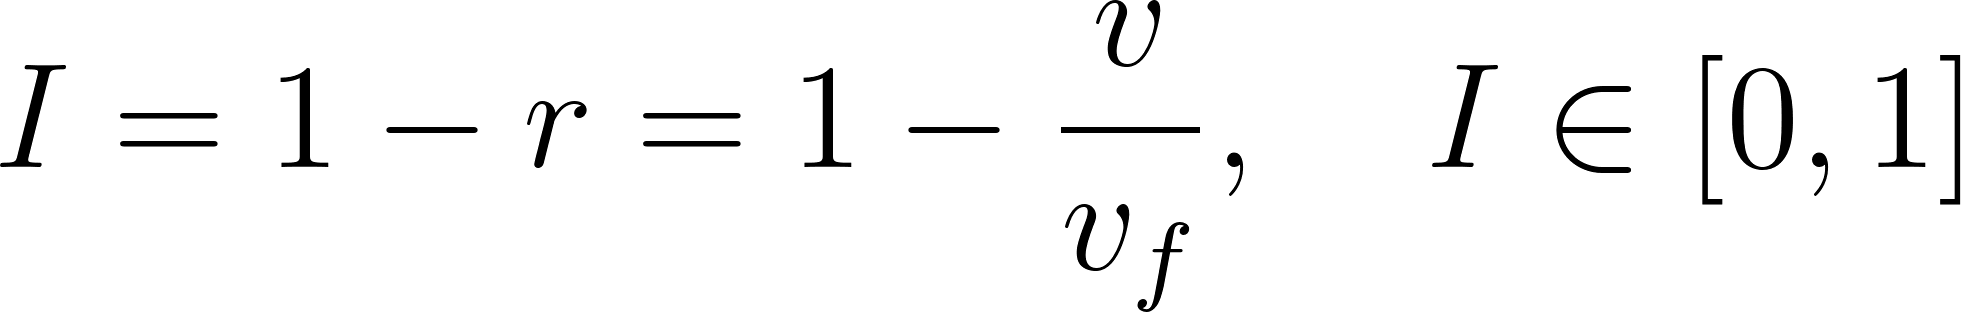
\includegraphics[width=0.5\linewidth]{Images/image5.png}
\end{center}

Độ trễ hành trình (Delay Seconds - $\Delta t$ ): Là phần thời gian chênh lệch mà phương tiện phải đánh đổi do sự suy giảm tốc độ.

\begin{center}

\includegraphics[width=0.5\linewidth]{Images/image14.png}
\end{center}

Phân cấp Mức độ Phục vụ (Level of Service - LOS): Dữ liệu định lượng (I) được rời rạc hóa (discretization) thành các nhãn định tính (từ A đến F) thông qua hệ luật chuyên gia (Rule-based mapping), lưu vào cột los\_level. Ví dụ: LOS A biểu thị dòng xe di chuyển tự do ($I \leq 0.15$), trong khi LOS F biểu thị trạng thái vỡ trận/tắc nghẽn nghiêm trọng ($I > 0.8$). Bước này rất quan trọng để hỗ trợ hệ thống Dashboard hiển thị màu cảnh báo tự động.

\subsubsubsection{Bài toán Ước lượng Lưu lượng bằng Nghịch đảo Hàm BPR}
API của TomTom không cung cấp trực tiếp lưu lượng xe (Volume). Để lấp đầy khoảng trống dữ liệu này cho cột pcu\_volume trong bảng fact\_traffic\_flow, hệ thống đã áp dụng kỹ thuật xấp xỉ toán học thông qua hàm BPR (Bureau of Public Roads) nổi tiếng trong kỹ thuật giao thông.


Hàm BPR nguyên thủy mô tả sự gia tăng thời gian di chuyển dựa trên tỷ số giữa lưu lượng và công suất (q/C):

\begin{center}
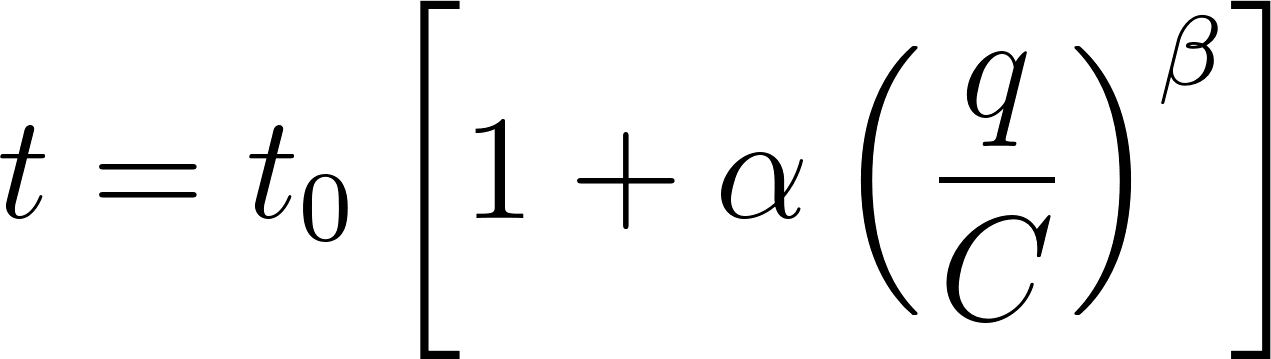
\includegraphics[width=0.3\linewidth]{Images/image8.png}
\end{center}

\begin{itemize}
    \item $t$: Thời gian hành trình thực tế (Current Travel Time).

    \item $t_0$: Thời gian hành trình thông thoáng (Free-flow Travel Time).

    \item $q$: Lưu lượng dòng xe cần tìm (Volume - PCU/h).

    \item $C$: Công suất thiết kế của đoạn đường (Capacity), hệ thống tính bằng:

    \[
    C = n_{lane} \times 2000
    \]

    \item $\alpha, \beta$: Các hệ số hiệu chuẩn
    (thường mặc định là $\alpha = 0.15, \beta = 4.0$).
\end{itemize}

Vì dữ liệu thu thập được là vận tốc, hệ thống thực hiện xấp xỉ \[
\frac{t}{t_0} \approx \frac{v_f}{v}
\] và nghịch đảo hàm BPR để tìm ra lưu lượng (q):

\begin{center}
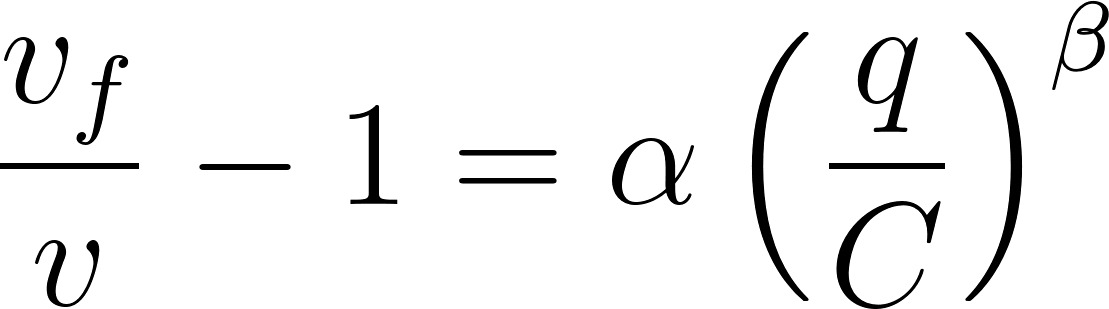
\includegraphics[width=0.3\linewidth]{Images/image12.png}
\end{center}

\begin{center}
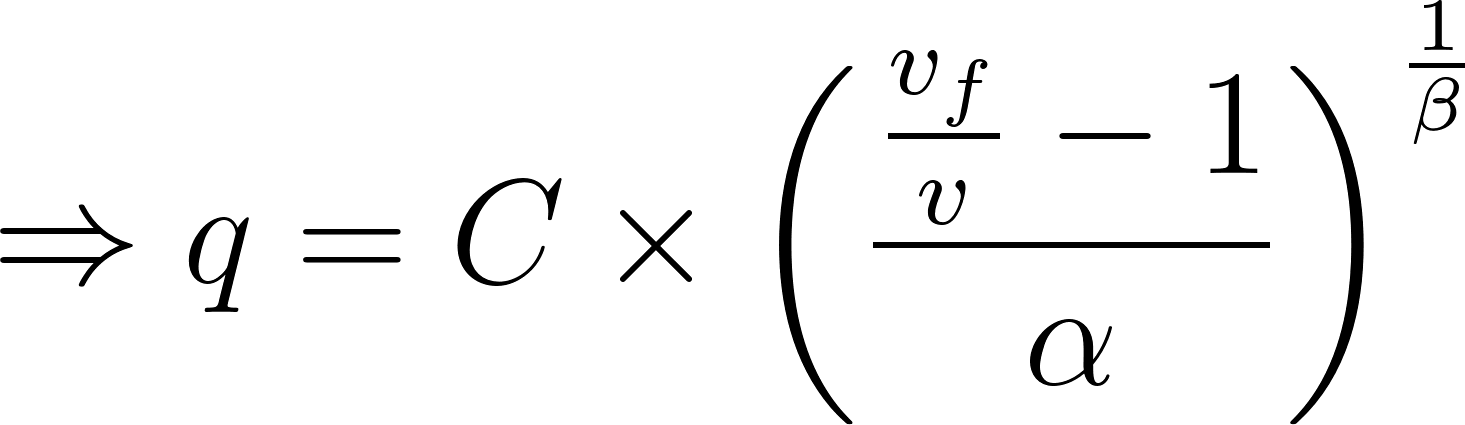
\includegraphics[width=0.3\linewidth]{Images/image27.png}
\end{center}

Để đảm bảo tính ổn định số học trong môi trường production, luồng Transform áp dụng các hàm chặn (guard-rails):


\begin{center}

\includegraphics[width=0.5\linewidth]{Images/image28.png}
\end{center}

Trong đó, $p_{max}$ (max\_vc\_ratio) là ngưỡng chặn trên (thường là 1.0 hoặc 1.2). Kỹ thuật này ngăn chặn hiện tượng tràn số (Overflow) hoặc rác dữ liệu sinh ra khi vận tốc v tiến dần về 0 trong các tình huống kẹt xe nghiêm trọng.


\subsubsection{Xử lý không gian và thuật toán khớp bản đồ}
Đối với luồng sự cố giao thông (incident\_pipeline.py), dữ liệu đầu vào là các tọa độ rời rạc (Latitude, Longitude) nằm trên hệ quy chiếu WGS84. Bài toán đặt ra là làm thế nào để "neo" (snap) các tọa độ này vào chính xác một đoạn đường (segment\_key thuộc bảng dim\_segment) để phân tích nguyên nhân - kết quả.


\subsubsubsection{Truy vấn K-Nearest Neighbors (KNN) với PostGIS}
Hệ thống giải quyết bài toán Map Matching bằng cách tận dụng sức mạnh của hệ cơ sở dữ liệu không gian PostGIS. Thay vì viết các vòng lặp tính khoảng cách Haversine kém hiệu quả trên Python, thuật toán sử dụng trực tiếp toán tử <-> (KNN - K-Nearest Neighbors) của PostgreSQL.


\begin{lstlisting}[language=SQL]
SQLSELECT ds.segment_key, ds.location_keyFROM dim_segment dsWHERE ds.geometry_center IS NOT NULLORDER BY ds.geometry_center <-> ST_SetSRID(ST_MakePoint(:lon, :lat), 4326)LIMIT 1
\end{lstlisting}

Về mặt độ phức tạp thuật toán, toán tử <-> khai thác triệt để cấu trúc cây R-Tree của chỉ mục không gian (GiST Index) idx\_dim\_segment\_center\_gist. Nó so sánh khoảng cách giữa tọa độ sự cố với các hộp giới hạn (Bounding Boxes) của đoạn đường, giúp giảm độ phức tạp tìm kiếm từ O(N) (Full Table Scan) xuống mức O(log N), đáp ứng hoàn hảo yêu cầu xử lý thời gian thực.

\subsubsubsection{Tiền xử lý hình học đa dạng (Geometry Preprocessing)}
Trong trường hợp sự cố (Incident) trả về hình dạng là một tuyến kéo dài (LineString) thay vì một điểm (Point), BaseTransformer sẽ thực hiện nội suy tọa độ trọng tâm (Centroid) trên bộ nhớ Python:


\begin{lstlisting}[language=SQL]
centroid_lon, centroid_lat = linestring_centroid(geom.coordinates)
\end{lstlisting}

Sau đó, nó được ép kiểu về định dạng Well-Known Text (WKT) POINT(lon lat) để BaseLoader sử dụng hàm ST\_GeomFromText(..., 4326) nạp chuẩn xác vào cột geometry kiểu geometry(Point,4326) trong bảng phân vùng fact\_incident.


\subsubsection{Chuẩn hóa ngữ nghĩa và phân rã chiều thời gian}
Để tương thích tuyệt đối với mô hình Snowflake Schema, mọi sự kiện phát sinh đều phải được phân rã khóa thời gian.


Đồng bộ múi giờ (Timezone Alignment): Mọi chuỗi ISO 8601 trả về từ API đều được phân tích cú pháp (parsing) và ép buộc (localize) về múi giờ chuẩn của hệ thống là Asia/Ho\_Chi\_Minh (UTC+7). Điều này triệt tiêu sai số thời gian khi phân tích các sự kiện xảy ra quanh ngưỡng nửa đêm.


Phân rã trục thời gian: Dấu thời gian (Timestamp) được bóc tách thành hai khóa ngoại (Foreign Keys) riêng biệt:


date\_key (Định dạng số nguyên YYYYMMDD): Dùng để liên kết với bảng dim\_date và đóng vai trò là khóa phân vùng (Partition Key) cho các bảng Fact.


time\_key (Số phút tích lũy trong ngày): Được tính bằng công thức
\[
\text{time\_key} = 60 \times \text{hour} + \text{minute}
\]
(thuộc miền giá trị \([0,1439]\)).

Việc ánh xạ sang \texttt{dim\_time\_of\_day} với độ phân giải tính bằng phút giúp Data Warehouse dễ dàng thực hiện các phép Roll-up (tổng hợp dữ liệu) theo khung 5 phút, 15 phút hoặc theo Ca trực (Shift) mà không cần dùng đến các hàm xử lý chuỗi thời gian nặng nề.

Chuẩn hóa Mức độ nghiêm trọng (Severity): Mức độ sự cố từ nhà cung cấp được ánh xạ tịnh tiến vào miền giá trị [0,4] thông qua hàm normalize\_magnitude(), đảm bảo sự đồng nhất ngữ nghĩa khi truy vấn dữ liệu từ nhiều nguồn khác nhau (như TomTom, OpenWeather, hay mạng xã hội).


\subsubsection{Kết luận}
Pha Transform trong kiến trúc hệ thống không chỉ là bước "làm sạch" dữ liệu thông thường, mà là một khối phân tích chuyên sâu (Analytical Engine). Bằng việc tích hợp các mô hình toán học (nghịch đảo BPR) và sức mạnh của đại số không gian (PostGIS KNN), lớp Transformer đã thành công trong việc "chiết xuất" các giá trị tri thức ẩn (như lưu lượng xe quy đổi PCU, hay vị trí vật lý đích xác của sự cố) từ những byte dữ liệu thô. Sự kết hợp giữa nguyên lý Hàm thuần túy trên Python và xử lý đồ thị không gian dưới Database tạo ra một luồng dữ liệu vừa có tính toàn vẹn cao, vừa mang ý nghĩa nghiệp vụ sâu sắc để phục vụ cho các mô hình Dự báo (Machine Learning) ở các bước tiếp theo.


\subsection{Kỹ thuật tối ưu hóa kho dữ liệu}
\subsubsection{Mục tiêu tối ưu hóa}
Trong hệ thống Traffic IoC, Data Warehouse không chỉ đóng vai trò lưu trữ tĩnh mà phải tiếp nhận luồng dữ liệu thời gian thực với tần suất cao (chu kỳ 15 phút/lần). Đặc thù này đặt ra ba thách thức lớn cho hệ quản trị PostgreSQL:


Write Amplification (Khuếch đại ghi): Khối lượng thao tác INSERT/UPDATE khổng lồ và liên tục có thể gây nghẽn cổ chai I/O (I/O Bottleneck).


Query Latency (Độ trễ truy vấn): Yêu cầu bóc tách dữ liệu theo cả hai chiều: Không gian (Spatial) và Thời gian (Temporal) trên các bảng Fact chứa hàng triệu bản ghi.


Table Bloat (Phình to dữ liệu): Đặc thù của cơ chế MVCC (Multi-Version Concurrency Control) trong PostgreSQL sinh ra các bản ghi rác (dead tuples) khi thực hiện cập nhật.


Để giải quyết triệt để các vấn đề này, hệ thống áp dụng một chiến lược tối ưu hóa toàn diện, kết hợp giữa Phân mảnh dữ liệu vật lý (Partitioning), Chỉ mục đa hình (Polymorphic Indexing) và Cơ chế ghi lũy đẳng.


\subsubsection{Chiến lược phân mảnh dữ liệu chuỗi thời gian}
Thay vì lưu trữ toàn bộ sự kiện giao thông vào một bảng nguyên khối (Monolithic Table) duy nhất, kiến trúc sư dữ liệu đã quyết định áp dụng kỹ thuật Range Partitioning (Phân vùng theo khoảng) dựa trên khóa phân vùng date\_key. Kỹ thuật này được áp dụng nhất quán trên các bảng sự kiện lõi như fact\_traffic\_flow, fact\_incident, và fact\_traffic\_risk\_prediction.


\begin{lstlisting}[language=SQL]
CREATE TABLE public.fact_traffic_flow (
    traffic_flow_key bigint NOT NULL,
    segment_key bigint NOT NULL,
    time_key integer NOT NULL,
    date_key integer NOT NULL,
) PARTITION BY RANGE (date_key);

CREATE TABLE public.fact_traffic_flow_202603 ( ... );

ALTER TABLE ONLY public.fact_traffic_flow
    ATTACH PARTITION public.fact_traffic_flow_202603
    FOR VALUES FROM (20260301) TO (20260401);
\end{lstlisting}

Về mặt nguyên lý hệ thống, kỹ thuật này mang lại các đột phá kiến trúc sau:


Partition Pruning (Cắt tỉa phân vùng): Khi một truy vấn (Query) từ Dashboard yêu cầu lấy dữ liệu lưu lượng của một ngày cụ thể, Query Planner của PostgreSQL sẽ tự động bỏ qua các phân vùng không liên quan. Điều này chuyển đổi độ phức tạp từ việc quét toàn bộ dữ liệu (Full Table Scan) sang chỉ quét trên một tập dữ liệu vật lý cực kỳ nhỏ.


Tối ưu hóa quản trị bộ nhớ (Memory Management): Hệ điều hành máy chủ chỉ cần nạp (cache) các phân vùng của tháng hiện tại ("Hot Data") vào bộ nhớ RAM, đẩy các phân vùng của các tháng trước ("Cold Data") xuống ổ cứng, giúp tối ưu hóa Cache Hit Ratio một cách tuyệt đối.


\subsubsection{Chiến lược đánh chỉ mục đa hình}
Lược đồ cơ sở dữ liệu (Database Schema) của dự án thể hiện sự am hiểu sâu sắc về cấu trúc dữ liệu bên dưới DBMS. Thay vì lạm dụng chỉ mục B-Tree mặc định, hệ thống triển khai một ma trận chỉ mục phức hợp để đáp ứng chính xác từng loại tải công việc (Workload).


\subsubsubsection{Chỉ mục không gian GiST (Generalized Search Tree)}
Đối với các trường dữ liệu mang tính chất tọa độ hình học (kiểu geometry(Point,4326) trong PostGIS), cấu trúc B-Tree truyền thống (vốn chỉ sắp xếp dữ liệu 1 chiều) hoàn toàn vô dụng. Hệ thống bắt buộc phải sử dụng GiST Index.


\begin{lstlisting}[language=SQL]
CREATE INDEX idx_fact_incident_geom_gist ON ONLY public.fact_incident
    USING gist (geometry);

CREATE INDEX idx_dim_segment_center_gist ON public.dim_segment
    USING gist (geometry_center);
\end{lstlisting}

GiST hoạt động dựa trên nguyên lý của cây R-Tree, chia không gian thành các Hộp giới hạn (Bounding Boxes) lồng nhau. Nhờ GiST, các truy vấn Map Matching sử dụng toán tử K-Nearest Neighbor (<->) có thể đạt tốc độ \$O(\textbackslash\{\}log N)\$ thay vì quét tuần tự.


\subsubsubsection{Chỉ mục khối dải BRIN (Block Range Index)}
Đây là một kỹ thuật tối ưu hóa bậc cao dành riêng cho dữ liệu Time-series. Cột timestamp và inserted\_at trong các bảng Fact mang đặc tính "chỉ chèn thêm" (append-heavy) và tăng dần theo thời gian.


\begin{lstlisting}[language=SQL]
CREATE INDEX idx_fact_traffic_flow_ts_brin ON ONLY public.fact_traffic_flow
    USING brin ("timestamp") WITH (pages_per_range='32');
\end{lstlisting}

Nếu dùng B-Tree, hệ thống phải lưu trữ index cho từng dòng (row), làm kích thước index có thể phình to ngang ngửa kích thước bảng. Ngược lại, BRIN Index chỉ lưu trữ giá trị cực tiểu (MIN) và cực đại (MAX) cho mỗi khối dữ liệu (ví dụ: mỗi 32 pages). Khi truy vấn theo dải thời gian, DBMS kiểm tra xem khoảng thời gian yêu cầu có giao (overlap) với MIN-MAX của khối hay không. Điều này giúp BRIN có kích thước cực kỳ nhỏ (chỉ vài Kilobytes) nhưng lại mang tốc độ lọc dữ liệu chuỗi thời gian tương đương B-Tree.


\subsubsubsection{Chỉ mục một phần (Partial Index) hỗ trợ Alerting}
Để phục vụ hệ thống giám sát và cảnh báo thời gian thực (Real-time Dashboards) mà không gây tốn kém dung lượng lưu trữ, lược đồ sử dụng kỹ thuật Partial Index.


\begin{lstlisting}[language=SQL]
CREATE INDEX idx_fact_incident_severe ON ONLY public.fact_incident
    USING btree (severity_level, segment_key)
    WHERE (severity_level >= 4);

CREATE INDEX idx_fact_flow_bad_los ON ONLY public.fact_traffic_flow
    USING btree (los_level, segment_key)
    WHERE (los_level = ANY (ARRAY['E'::bpchar, 'F'::bpchar]));
\end{lstlisting}

Kiến trúc này cho phép PostgreSQL tạo ra một cây chỉ mục với kích thước cực nhỏ (chỉ chứa các điểm đen giao thông). Các truy vấn đếm số lượng điểm ùn tắc từ Dashboard sẽ quét thẳng vào Partial Index này và trả về kết quả gần như tức thời (sub-millisecond latency).


\subsubsection{Cơ chế UPSERT và Quản lý "Bloat" trong MVCC}
Tại tầng BaseLoader, hệ thống sử dụng cú pháp INSERT ... ON CONFLICT DO UPDATE (UPSERT) để bảo toàn tính lũy đẳng (Idempotency). PostgreSQL dựa vào các Ràng buộc Khóa chính (Primary Key Constraints) được định nghĩa chặt chẽ trên từng phân vùng vật lý để phát hiện xung đột:


\begin{lstlisting}[language=SQL]
ALTER TABLE ONLY public.fact_traffic_flow_202603
    ADD CONSTRAINT fact_traffic_flow_202603_pkey
    PRIMARY KEY (traffic_flow_key, date_key);
\end{lstlisting}

Mặc dù UPSERT bảo vệ hệ thống khỏi rác dữ liệu trùng lặp (duplicates), quá trình cập nhật đè lên bản ghi cũ trong PostgreSQL sẽ đánh dấu row cũ là "dead tuple", gây ra hiện tượng phình to dữ liệu (Table Bloat) do cơ chế quản lý giao dịch MVCC.


Sự kết hợp giữa UPSERT và Table Partitioning chính là "chìa khóa" giải quyết vấn đề này. Nhờ việc dữ liệu bị băm nhỏ thành từng tháng, tiến trình dọn dẹp tự động (Auto-vacuum) của PostgreSQL chỉ cần tập trung quét dọn các "dead tuples" sinh ra trong phân vùng của tháng hiện tại (Active Partition) thay vì phải chật vật quét toàn bộ kho dữ liệu nhiều năm. Điều này triệt tiêu hoàn toàn chi phí bảo trì hệ thống và đảm bảo hiệu năng I/O luôn ở trạng thái tốt nhất.


\subsubsection{Kết luận}
Chiến lược thiết kế cơ sở dữ liệu của dự án minh chứng cho sự kết hợp hài hòa giữa cấu trúc vật lý và logic nghiệp vụ. Việc lựa chọn khéo léo các phương pháp lập chỉ mục thế hệ mới (BRIN cho chuỗi thời gian, GiST cho không gian hình học, Partial Index cho cảnh báo nghiệp vụ) kết hợp với kỹ thuật phân mảnh Range Partitioning đã tạo ra một Data Warehouse "miễn nhiễm" với các giới hạn về độ lớn của bộ nhớ. Đây là một nền tảng vững chắc, vừa tối ưu hóa tốc độ ghi (write-optimized) trong các chu kỳ ETL 15 phút, vừa đảm bảo khả năng phản hồi tốc độ cao (read-optimized) cho các ứng dụng hiển thị và phân tích đầu cuối.
